\chapter{A Semi-Lagrangian Method for Detecting and Tracking \acrshort{dcc}s in Geostationary Satellite Observations} \label{chp:tracking_method}


\section{Introduction} %% \introduction[modified heading if necessary]


Sequences of images from satellite instruments have been used to detect and track the motion of \acrshort{dcc}s and tropical storms since the earliest geostationary weather satellites \citep{menzel_cloud_2001}.
Whereas early detection and tracking were performed by hand, numerous algorithms have been developed to perform this task automatically, and are widely used for both forecasting and research purposes (section~\ref{sec:tracking_timeline}).
There is a continual effort both to improve existing algorithms and develop new methods to support these activities.
However, it is important to understand the differences in observations of \acrshort{dcc}s from satellite imagery to those of other sources, particularly radar and lightning observations.

Visible and \acrshort{ir} imagery from modern geostationary weather satellite instruments provide unique observations of \acrshort{dcc}s and their surrounding environment.
Figure~\ref{fig:compare_sat_radar_glm} compares observations of \acrshort{dcc}s throughout three different stages of their lifecycle between satellite visible and \acrshort{ir} imagery, doppler cloud radar and lightning flash observations.
Composite \acrfull{rgb} images from a combination of visible and \acrshort{nir} channels aboard the \acrfull{abi} show a.: small, isolated cores during the growing phase; b.: a large area of optically thick anvil during the mature phase, and c.: a large area of optically thin anvil cloud during the dissipating phase.
\acrshort{bt} imagery from the \acrshort{abi} 10.4\,\unit{\mu m} channel displays d.: cold, small, developing cores; e.: a large, cold anvil cloud, and f.: warmer \acrshort{bt}s caused by thermal radiation from the surface penetrating the optically thin dissipating anvil. 
Lightning flash locations observed by the \acrfull{glm} aboard \acrshort{goes}-16 show g.: low frequency during the growing phase; h.: high frequency during the mature phase, and i.: no lightning activity in the dissipating phase. 
Column mean radar reflectivity observed by \acrfull{nexrad} Doppler cloud radar shows high radar reflectivity in the convective cores during the j. growing and k. mature phases, and no area of high radar reflectivity during the dissipating phase. 
The outline of the region of \acrshort{bt}s below 270\,\unit{K} observed by \acrshort{abi} is shown by the orange dashed contour over the \acrshort{glm} flash locations and \acrshort{nexrad} radar reflectivity to indicate their observations relative to the anvil cloud.


%f
\begin{figure}[tp]
    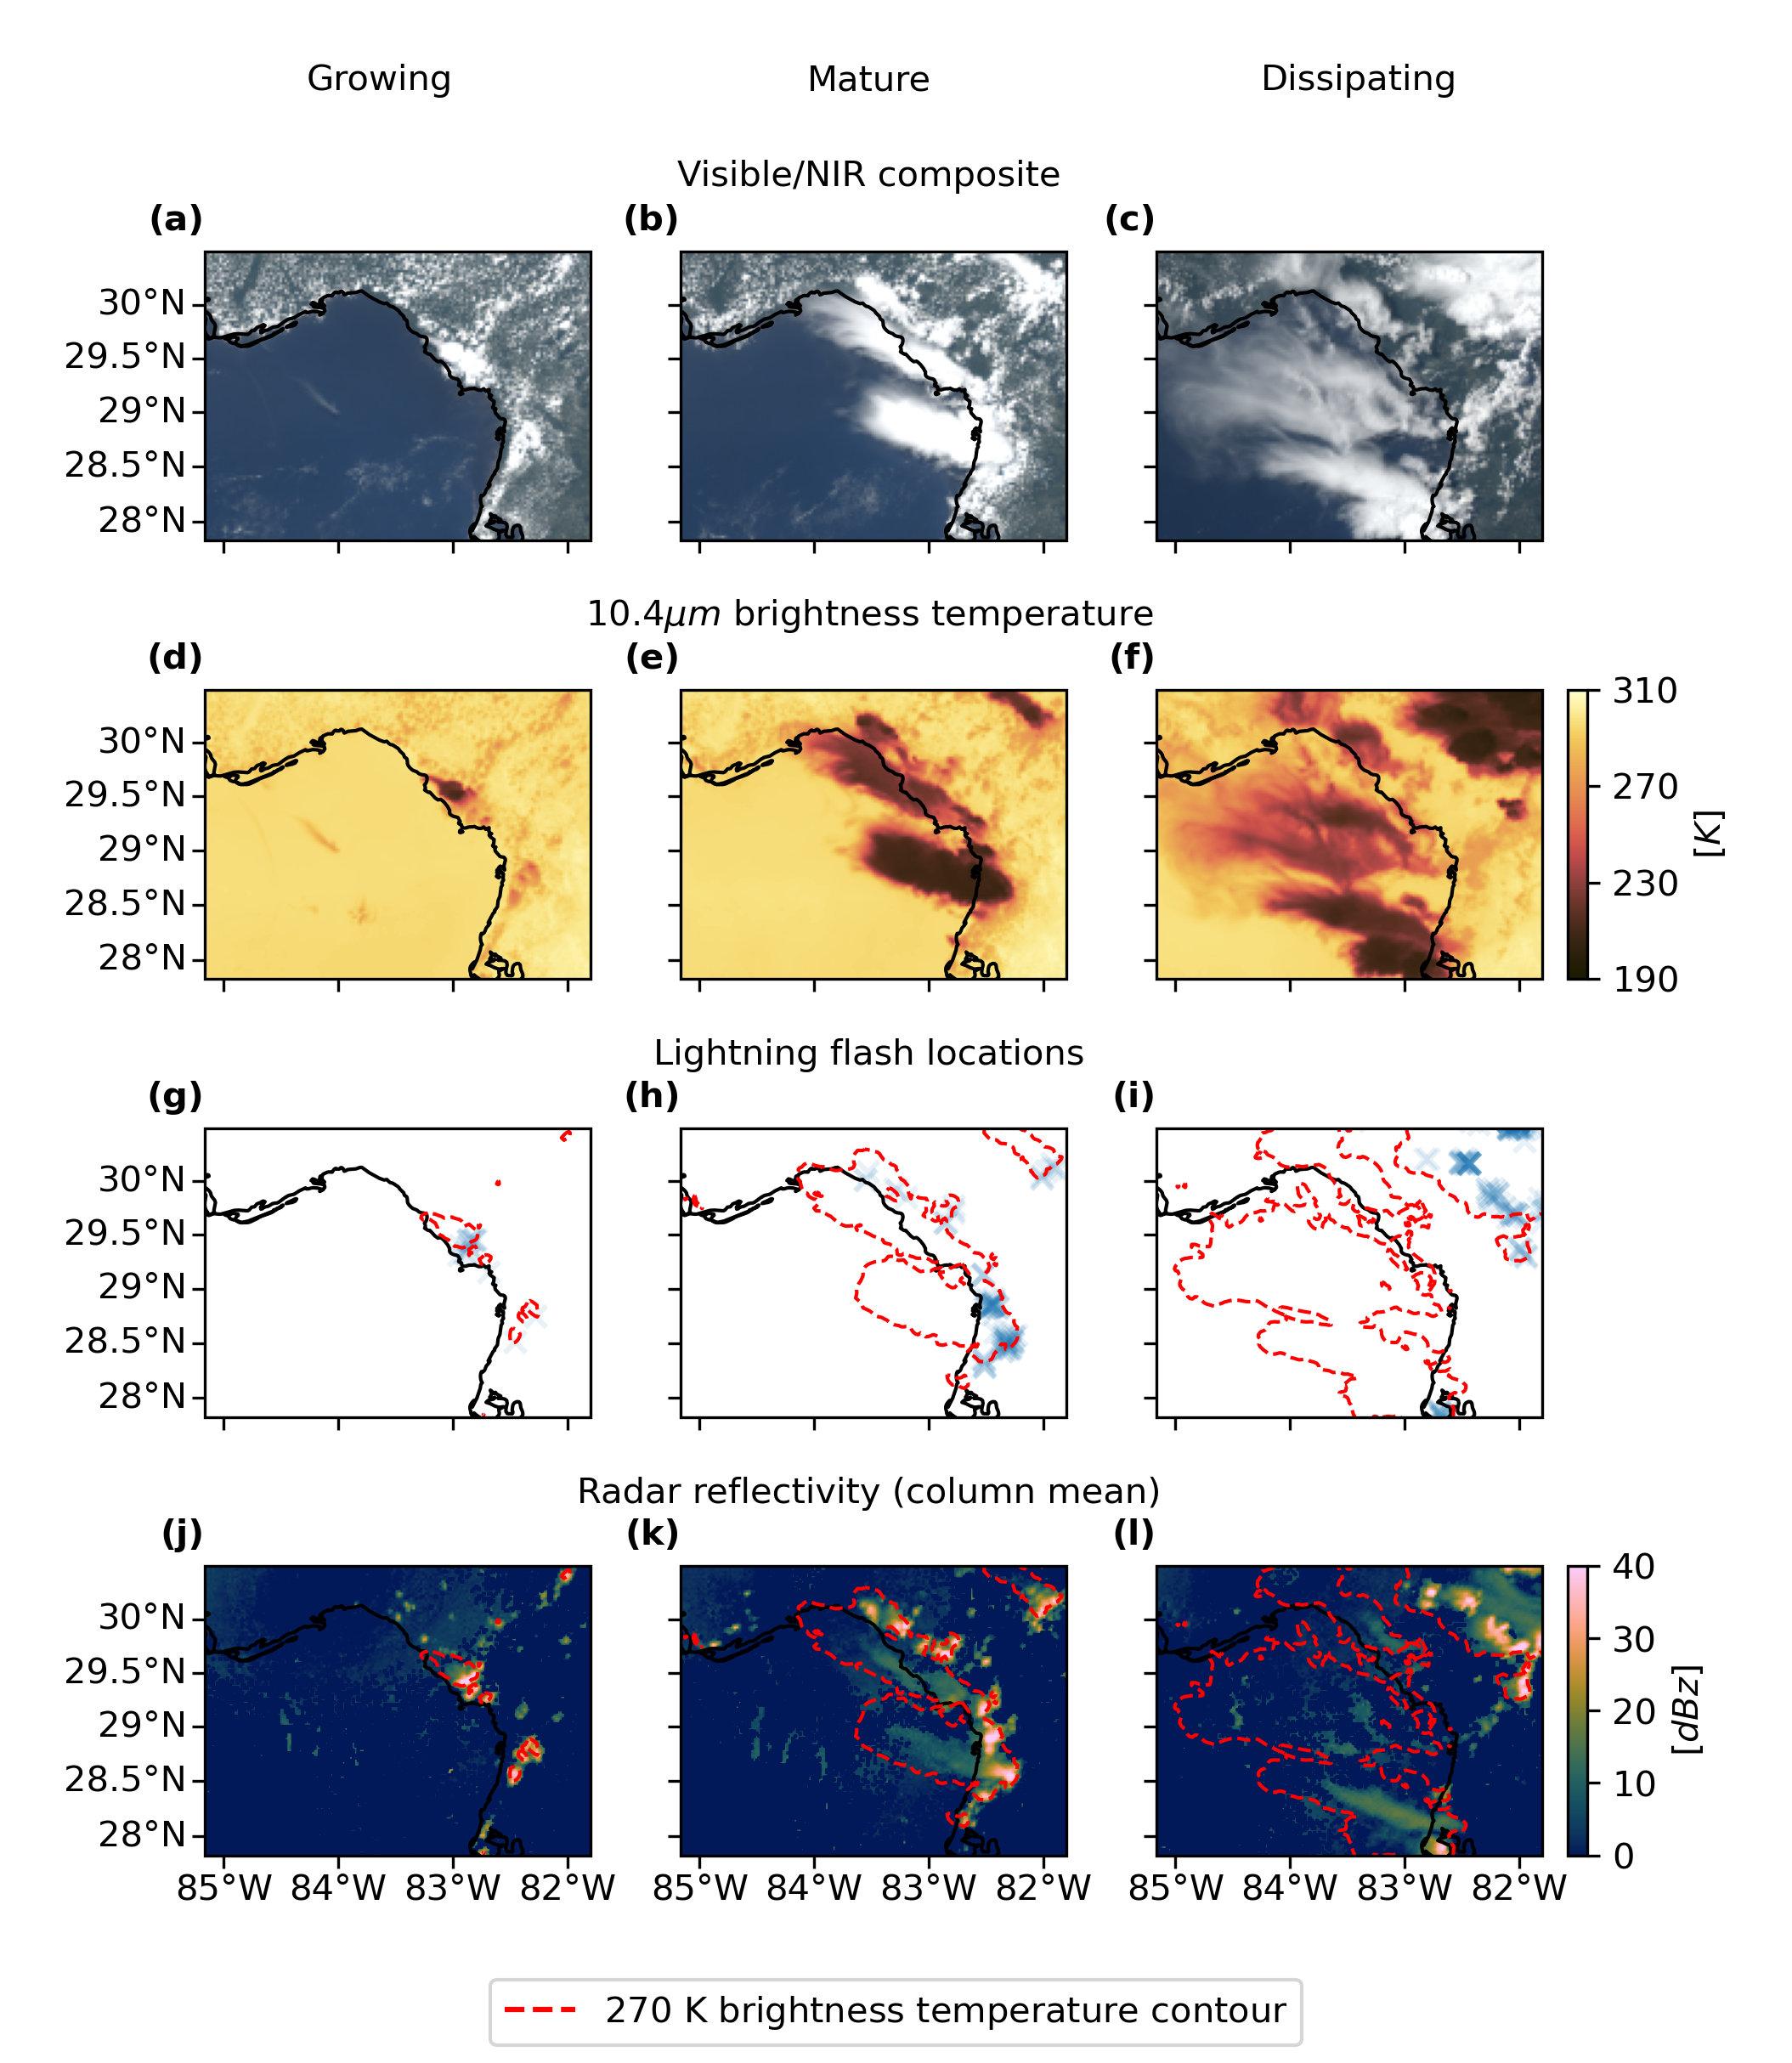
\includegraphics[width=\textwidth]{figures/chapter1_01.png}
    \caption[
    Observations of a cluster of \acrshort{dcc}s over North-West Florida throughout three stages of their lifecycle
    ]{
    Observations of a cluster of \acrshort{dcc}s over North-West Florida throughout three stages of their lifecycle. This cluster of \acrshort{dcc}s occurred on the afternoon of 19\textsuperscript{th} June 2018. The `growing' column was observed at 17:00 \acrshort{utc}, the `mature' column at 19:00 \acrshort{utc}, and the `dissipating' column at 21:00 \acrshort{utc}. The four rows show observations of \acrshort{abi} visible/\acrshort{nir} composites (a,b,c), and 10.4\,\unit{\mu m} \acrshort{bt} (d,e,f); lightning flash locations observed by \acrshort{glm} (g,h,i), and column mean radar reflectivity observed by \acrshort{nexrad} (j,k,l). Note that, unless otherwise specified, this case study is used for all subsequent figures in this chapter.
    }
    \label{fig:compare_sat_radar_glm}
\end{figure}


These instruments are capable of observing the extent of the anvil clouds associated with \acrshort{dcc}s over their entire lifecycle, even after convective activity has ceased (fig.~\ref{fig:compare_sat_radar_glm}\,f).
This is of particular importance due to the influence of anvil cloud radiative forcing on the climate, their response to temperature change \citep{bony_thermodynamic_2016, hartmann_tropical_2016, ceppi_cloud_2017, gasparini_what_2019} and possible feedbacks on subsequent convective activity.
The newest generation of geostationary imaging satellites offers greater opportunities for the study of \acrshort{dcc}s due to their high spatial and temporal resolution -- allowing the detection and tracking of individual convective cores \citep{heikenfeld_tobac_2019} -- and also due to their high signal-to-noise ratio allowing research quality observations \citep{iacovazzi_goes-16_2020}.

The detection and tracking of \acrshort{dcc}s from satellite imagery remains challenging due to the inability to directly observe the convection that drives \acrshort{dcc}s using passive visible and \acrshort{ir} observations.
This is unlike radar and lightning observations, which can directly observe deep convection due to the strong correlations between core updraft intensity and radar reflectivity and polarisation \citep{austin_relation_1987,  zipser_vertical_1994},  and lightning flash occurrence \citep{williams_relationship_1989}.
Instead, a proxy for convective activity must be used to detect deep convection in visible/\acrshort{ir} satellite imagery.
The approaches used for this can generally be separated into two separate methods. 
Firstly, the use of thresholds on \acrshort{bt} or other observed fields, which are capable of detecting \acrshort{dcc} anvil clouds \citep[e.g.][]{schmetz_monitoring_1997, hong_detection_2005, schroder_deep_2009}.
Secondly, the detection of rapidly growing cloud tops by observing changes in the anvil cloud-top radiative cooling, or by other similar approximations of cloud growth \citep{zinner_cb-tram_2008, bedka_objective_2010}.

Developing a detection method using either approach is made challenging by the dynamic nature of \acrshort{dcc}s themselves.
\acrshort{dcc} cores typically have diameters of around 10\,\unit{km}, and updraft velocities on the order of 10\,\unit{m s\textsuperscript{-1}} \citep{weisman_mesoscale_2015}, and exist for 1-3 hours \citep{chen_diurnal_1997}.
Large, mesoscale convective systems (consisting of multiple cores joined by a single large anvil \citep{roca_simple_2017}) may span areas several orders of magnitude larger than isolated \acrshort{dcc}s \citep{houze_mesoscale_2004}, and typically exist to 10-20 hours or longer \citep{chen_diurnal_1997}.
The life cycle of a \acrshort{dcc} can be split into three phases: an initiation or growing phase, a mature phase and a dissipating phase after the cessation of convective activity \citep{wall_life_2018}.
There exists a significant difference between the diurnal cycles of deep convection over the land and over the ocean, with observed \acrshort{dcc}s over land clustered towards the end of the day \citep{taylor_evaluating_2017}.


%f
\begin{figure}[tp]
    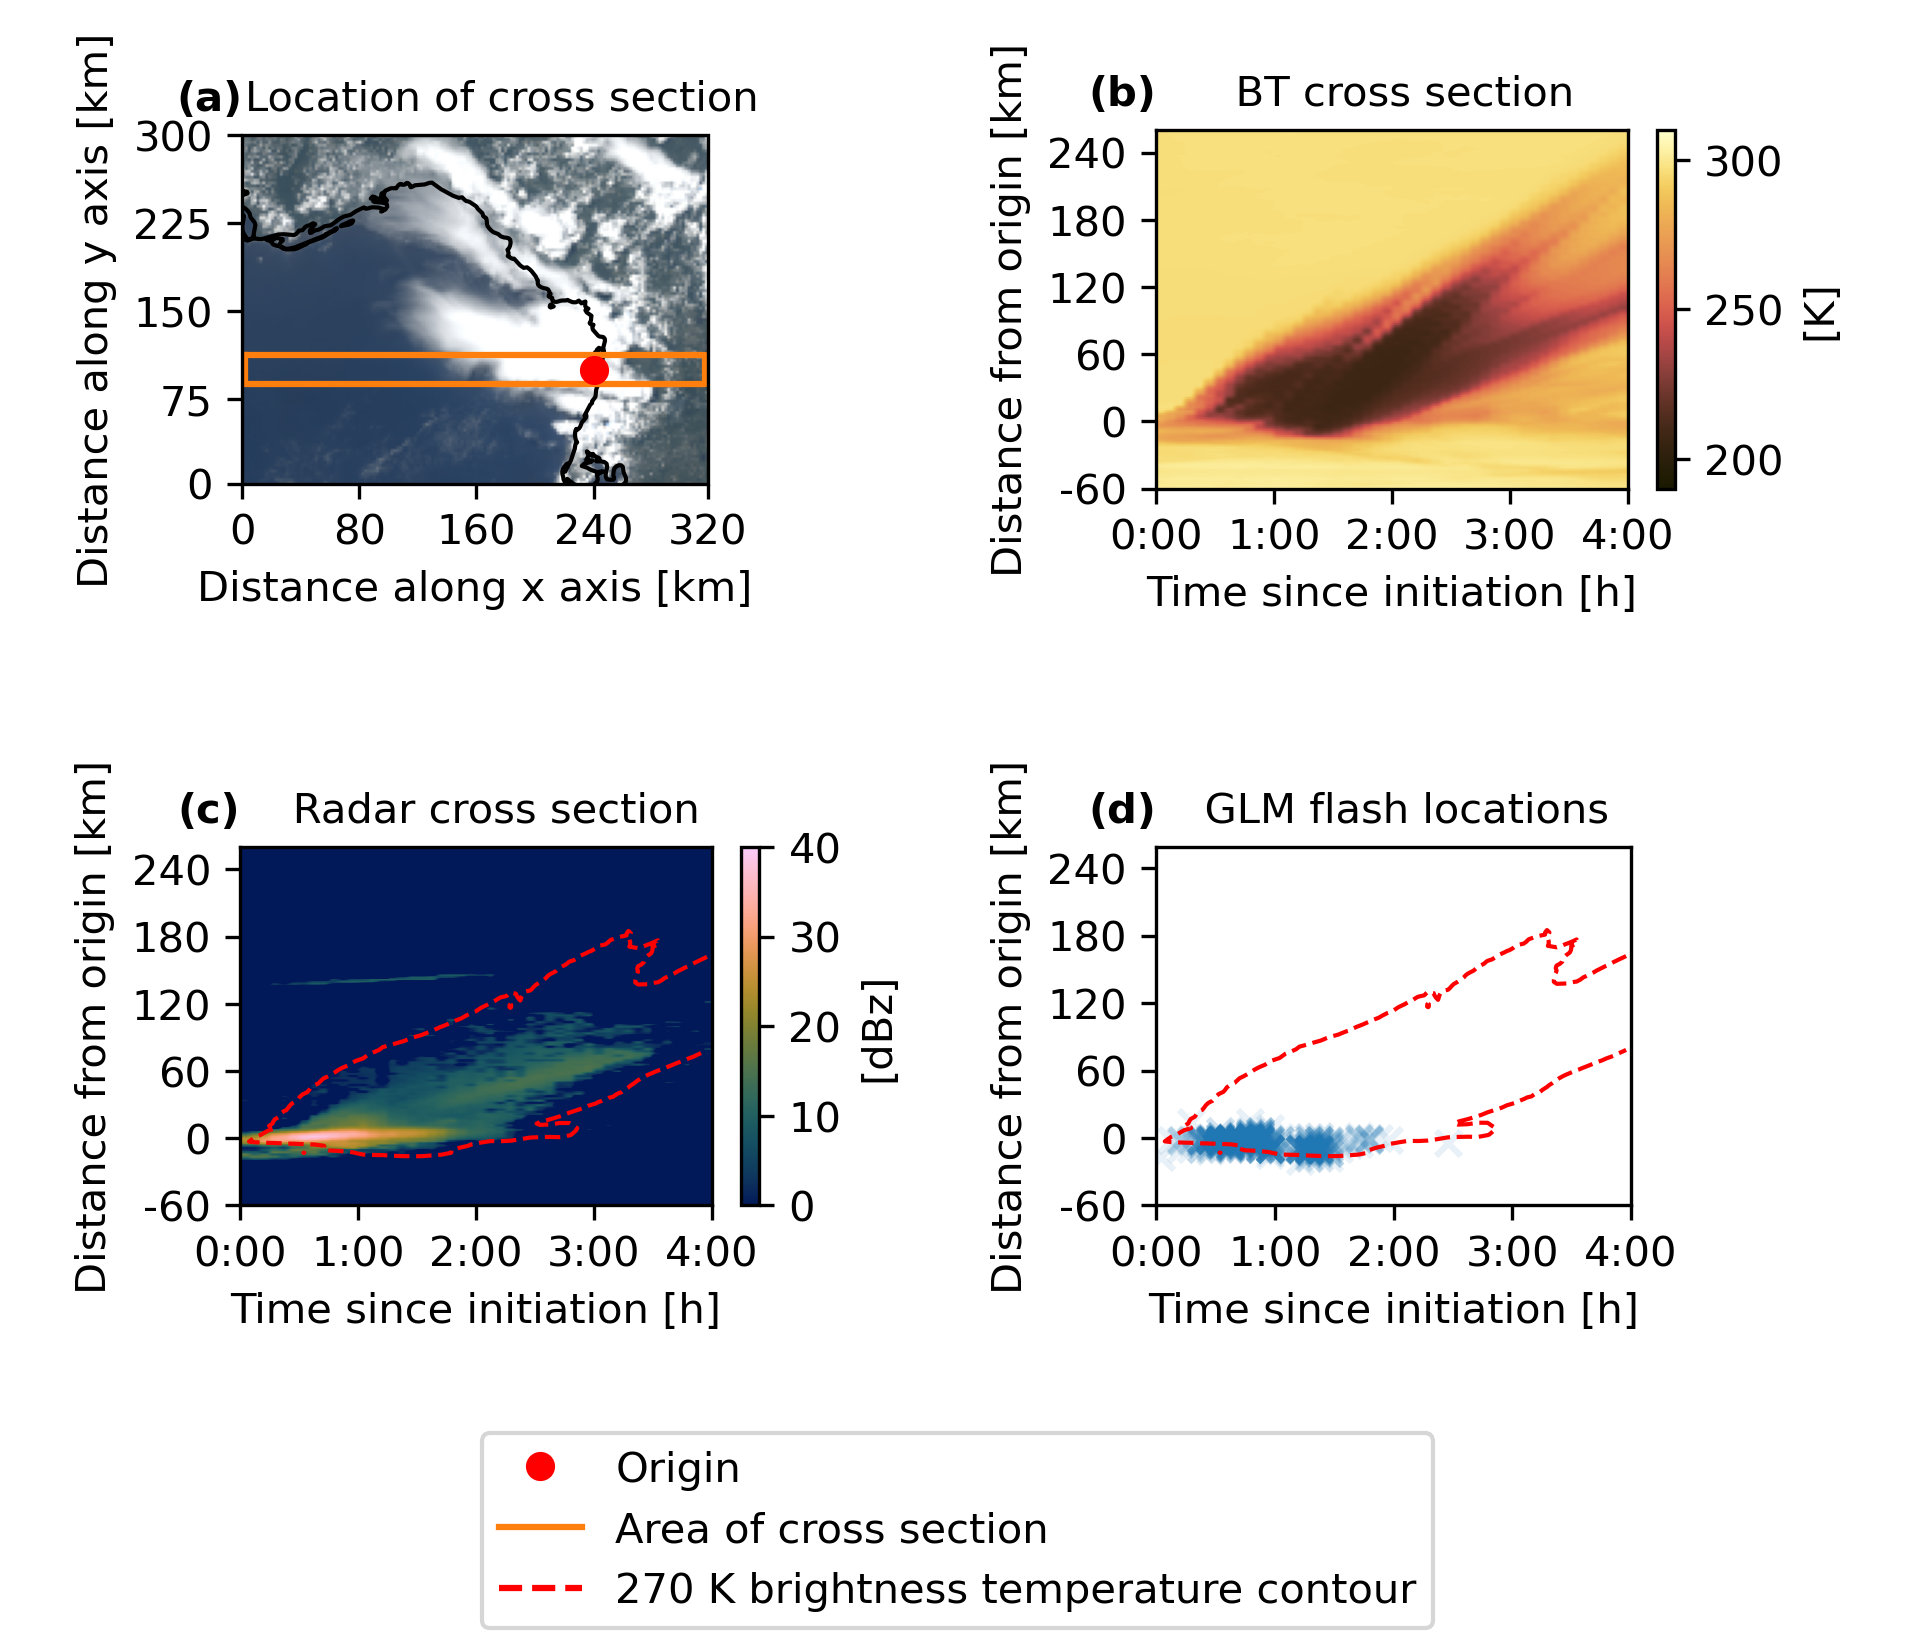
\includegraphics[width=\textwidth]{figures/chapter1_02.png}
    \caption[
    Cross sections of the \acrshort{dcc} observed in figure~\ref{fig:compare_sat_radar_glm} as they develop over time
    ]{
    Cross sections of the \acrshort{dcc} observed in figure~\ref{fig:compare_sat_radar_glm} as they develop over time. a.: The location of the cross-section within the observed \acrshort{dcc}. The mean of values is taken in the North-South axis. b.: \acrshort{abi} 10.8\,\unit{\mu m} \acrshort{bt}, showing rapid cooling for the first 30 minutes, followed by an expanding region of anvil cloud that begins to thin and warm after 2-3 hours. c.: Column mean radar reflectivity, showing the presence and location of the convective core. d.: Lightning flash locations observed by \acrshort{glm}, which closely match the core observed by \acrshort{nexrad}. Initiation occurred at 82.0\,\textdegree W 28.5\,\textdegree N at a time of 17:00 \acrshort{utc}.
    }
    \label{fig:dcc_over_time}
\end{figure}


The difficulties of detecting \acrshort{dcc}s using various proxy approaches are demonstrated by the cross-sections of an observed \acrshort{dcc} over time in fig.~\ref{fig:dcc_over_time}.
The observed \acrshort{bt} of the \acrshort{dcc} anvil cloud shows wide variation over time, with the anvil cloud thinning due to dissipation after the end of convective activity which results in a warmer \acrshort{bt} due to greater signal from the surface.
This variety of observed temperatures leads to large differences in the chosen threshold value between different algorithms \citep[see discussion in][]{bennartz_convective_2012}.
This choice of the threshold value is further complicated due to the overlap in observed \acrshort{bt}s between \acrshort{dcc} anvils and non-convective clouds \citep{konduru_new_2013}.
As a result, any detection method using a \acrshort{bt} threshold must compromise between missed detection of \acrshort{dcc}s, or false detections of non-\acrshort{dcc} clouds.

The cooling of the cloud top is only visible for a short period during the initial phase of the \acrshort{dcc}, before the anvil cloud top reaches the tropopause temperature after approximately 30 minutes.
As a result, any method that solely relies on detecting the growth of the \acrshort{dcc} will be unable to detect the anvil cloud after this initial growth phase has ended.
While such algorithms provide accurate detection of these early phases of \acrshort{dcc} growth \citep{zinner_validation_2013}, they are unable to continue tracking the anvil cloud after convective activity is no longer observed.

\citet{fiolleau_algorithm_2013} identified this need to compromise on the accuracy of detecting \acrshort{dcc}s as a problem caused by the commonly used two-step framework for detecting and tracking \acrshort{dcc}s.
In this framework, \acrshort{dcc}s are first detected in individual images, and then linked together over time in sequences of images.
As a result, the detection method chosen must be capable of detecting \acrshort{dcc}s at each individual time step in order to track their entire lifecycle.
Instead \citet{fiolleau_algorithm_2013} implemented a single-step framework for mesoscale convective systems that treats a sequence of images as a `3-D' volume (consisting of two spatial dimensions and one temporal dimension), and performs detection and tracking simultaneously by applying a watershed method over both spatial and temporal dimensions.
Whereas this approach was successful for large, mesoscale systems, where the advection of the anvil is small compared to the overall anvil area, it is less capable of tracking small, rapidly moving convective cores.
A semi-Lagrangian framework has been developed which allows for single-step detection and tracking which accounts for the motion of \acrshort{dcc}s using optical flow, improving the tracking of small \acrshort{dcc}s.

Utilising the semi-Lagrangian framework, the best elements of both growth-based and threshold-based detection methods can be combined.
It is possible to detect growing \acrshort{dcc}s to a high degree of accuracy using methods similar to those of \citet{zinner_cb-tram_2008}, and then extend the detected \acrshort{dcc} over the entire anvil cloud using the 3-D watershed method of \citet{fiolleau_algorithm_2013}.
This framework reduces the compromise required between the rate of missed \acrshort{dcc}s and falsely detected \acrshort{dcc}s, improving the overall accuracy of our detection method compared to existing approaches.
Furthermore, this method allows the anvil cloud to be detected and tracked even after the region of cloud top cooling is no longer detected.
Finally, the 3-D method handles the merging and splitting of intersecting \acrshort{dcc}s by detecting all \acrshort{dcc}s that intersect at any point during their lifetime as a merged object.


\section{Data}

Three sources of data are used throughout this chapter.
Primarily, visible and \acrshort{ir} imagery from \acrshort{abi} aboard the \acrshort{goes}-16 weather satellite is used for the detection of \acrshort{dcc}s.
Secondarily, observations from the \acrshort{nexrad} weather radar network and the \acrshort{glm} (also aboard \acrshort{goes}-16) are used to assess and validate the tracking and detection method presented here.


\subsection{Advanced Baseline Imager} \label{sec:abi_data}


The \acrshort{abi} is a visible and \acrshort{ir} radiometer aboard the \acrshort{goes}-16 series of weather satellites \citep{schmit_closer_2016}.
\acrshort{goes}-16, also known as \acrshort{goes}-East, is situated in a geostationary orbit at 75.2\,\textdegree W above the equator, providing a field of view (or `Earth-disc') covering most of the western hemisphere, including all of South America and most of North America.
\acrshort{abi} has 16 channels operating in a range of spectral bands in the visible, \acrshort{nir} and thermal-\acrshort{ir}.
The majority of these channels have a resolution of 2\,\unit{km} at the sub-satellite point, although this reduces to approximately 3\,\unit{km} across most of the \acrfull{conus} due to the satellite viewing angle.
\acrshort{abi} operates in a flexible scan mode, making observations of the \acrshort{conus} once every 5 minutes, the full disc every 10 minutes (15 minutes prior to April 2019), and two mesoscale regions of approximately 2500 by 2500\,\unit{km} every minute.
Additionally, it is capable of scanning the full disc every five minutes if no other scans are performed.
This combination of high spatial and temporal resolution makes \acrshort{abi} suitable for detecting and tracking small and developing \acrshort{dcc}s, as well as providing the spatial coverage to also track large mesoscale convective systems \citep{heikenfeld_tobac_2019}.


%t
\begin{table}[tb]
\centering
\begin{tabular}{lrrr}
\tophline
Instrument                                              & \acrshort{abi}   & \acrshort{seviri}    & Imager \\
\middlehline
Temporal resolution (\unit{minutes})                    & 5     & 15        & 30 \\
Nadir spatial resolution (\unit{k m})                   & 2     & 3         & 4 (8 for \acrshort{wv}) \\
Number of \acrshort{ir} \acrshort{lw} window channels                         & 3     & 2         & 2 \\
Number of \acrshort{ir} \acrshort{wv} channels                                & 3     & 2         & 1 \\
% Noise equivalent temperature  (\unit{K} @ 300\,\unit{K})  & 0.1   & 0.25      & 0.09 \\
\bottomhline
\end{tabular}
\caption[
Comparison of data from \acrshort{abi} to that from older geostationary instruments
]{
Comparison of data from \acrshort{abi} to that from older geostationary instruments\; \acrshort{seviri} aboard the second generation meteosat satellites, and the imager aboard the second generation \acrshort{goes}.
} % Table Footnotes
\label{table:abi_comparison}
\end{table}

Compared to older geostationary instruments, \acrshort{abi} has higher spatial and temporal resolution, and more channels in both the \acrshort{lw} \acrshort{ir} window spectrum and the \acrshort{lw} \acrshort{ir} \acrfull{wv} spectrum (table \ref{table:abi_comparison}) \citep{iacovazzi_goes-16_2020}.
This, combined with many of the channels being derived from those aboard the Visible Infrared Imaging Radiometer Suite, make the data from \acrshort{abi} more suitable for research purposes than that from older instruments \citep{heidinger_chapter_2020}.
Several artifacts are known to occur in \acrshort{abi} imagery \citep{gunshor_goes-r_2020}.
Although the majority of these artifacts are removed using the data quality flag associated with the \acrshort{abi} data, in a number of cases bad detector stripes (described in section 3.2 of \citealp{gunshor_goes-r_2020}) are not flagged in the data. 
These regions are detected separately, and replaced with missing data prior to cloud tracking.

In this chapter  \acrshort{abi} level 2 \acrfull{mcmip} is used, which provides calibrated reflectances and \acrshort{bt}s for all \acrshort{abi} channels on a common grid \citep{schmit_chapter_2020}, using the 5-minute frequency imagery provided over the \acrshort{conus} region.
The case study shown in the figures throughout this chapter is for a subset of the \acrshort{conus} scan region centred at 83.7\,\textdegree W, 29.2\,\textdegree N, over the time period of 17:00:00 to 21:00:00 \acrshort{utc} on the 19th June 2018.
Validation was performed on the \acrshort{conus} scan region over the entirety of 2018.
All data has been sourced through the \acrshort{noaa} Big Data Program.



\subsubsection{Selection of \acrshort{abi} Channels and Channel Combinations} \label{sec:abi_channels}

In order to have an equal performance during both day and nighttime, a selection of \acrshort{lw} \acrshort{ir} \acrshort{abi} channels are used for the detection and tracking of \acrshort{dcc}s (see fig.~\ref{fig:abi_channels}). 
These channels consist of the 10.4\,\unit{\mu m} and 12.4\,\unit{\mu m} \acrshort{lw} (also known as the clean and dirty window channels respectively due to the presence of \acrshort{wv} in the latter), and the upper and lower troposphere \acrshort{wv} channels at 6.2\,\unit{\mu m} and 7.3\,\unit{\mu m} respectively.
Whereas the \acrshort{lw} window \acrshort{ir} \acrshort{bt} is commonly used for the detection of anvil clouds using threshold-based methods, it is not used for this purpose in this method due to the wide range of \acrshort{bt}s observed within anvil clouds, and the variance of anvil cloud temperature with changes in tropopause temperature due to meteorology and latitude.
However, the information contained within this field is used for the optical flow calculation of the cloud motion field.


%f
\begin{figure}[tp]
    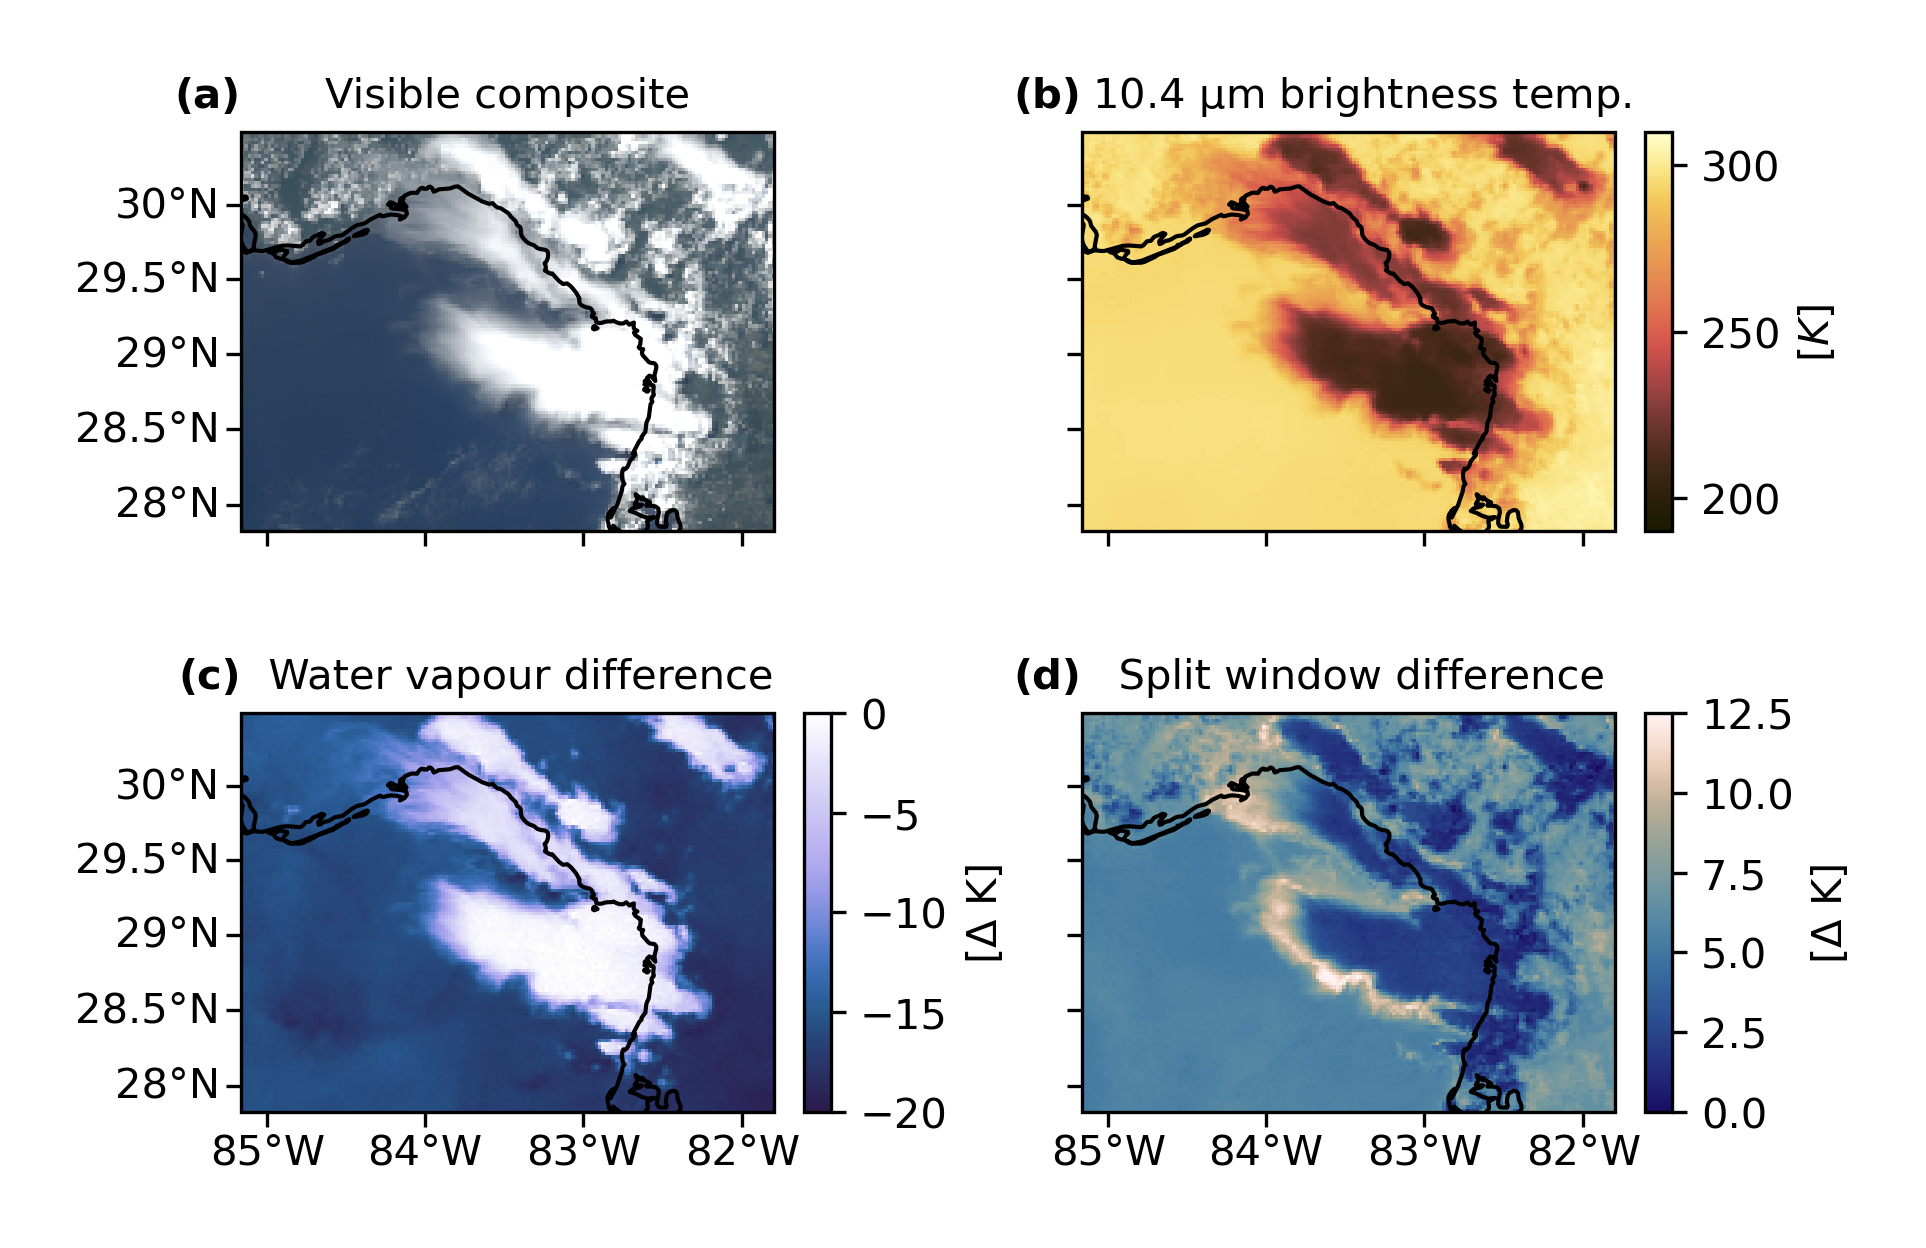
\includegraphics[width=\textwidth]{figures/chapter1_03.png}
    \caption[
    \acrshort{abi} channels and channel differences used with the detection and tracking algorithm
    ]{
    \acrshort{abi} channels and channel differences used with the detection and tracking algorithm. a.: A composite of visible and \acrshort{nir} channels. b.: The 10.4\,\unit{\mu m} \acrshort{bt}, or clean \acrshort{lw} window channel, which can differentiate clouds at all altitudes by their \acrshort{bt}. c.: the \acrshort{wvd} combination, of the 6.2\,\unit{\mu m} upper troposphere \acrshort{wv} channel minus the 7.3\,\unit{\mu m} lower troposphere \acrshort{wv} channel, which is strongly negative for clear sky and low cloud, but approaches positive values for thick, high clouds. d.: the \acrshort{swd} combination of the 10.4\,\unit{\mu m} clean \acrshort{lw} window channel minus the 12.4\,\unit{\mu m} dirty \acrshort{lw} window channel, which is near zero for thick clouds, around\,\unit{K} for clear skies and approximately 10\,\unit{K} for thin, ice clouds.
    }
    \label{fig:abi_channels}
\end{figure}


Two additional combinations of channels are used to detect areas of \acrshort{dcc} anvil. 
The \acrfull{wvd} combination (fig.~\ref{fig:abi_channels}\,c) of the upper troposphere \acrshort{wv} channel minus the lower troposphere \acrshort{wv} channel has been shown to provide a high detection rate for \acrshort{dcc}s \citep{muller_role_2018, muller_novel_2019}.
In clear sky or low cloud conditions, \acrshort{wvd} shows the temperature difference between the upper and lower troposphere of generally around -20\,\unit{K}. 
While the 6.2\,\unit{\mu m} has an additional contribution from stratospheric \acrshort{wv} \citep{schmetz_monitoring_1997}, this does not have a significant effect on the \acrshort{wvd} due to the small size of this absorption (fig.~\ref{fig:abi_vertical_weighting}.
Because both the \acrshort{wv} channels are strongly absorbed by \acrshort{wv} in the lower troposphere, the \acrshort{wvd} field is not affected by surface and low altitude features and so provides a clear distinction between thick, high clouds and the background across a wide range of situations.
\citet{muller_novel_2019} found that a threshold of -5\,\unit{K} gave a high detection rate of anvil clouds.
Furthermore, as the \acrshort{wvd} values are relative to the lower stratosphere temperatures, this field is much less affected by location and meteorology than the \acrshort{lw} \acrshort{ir} channels.
However, the \acrshort{wvd} is still prone to the false detections of non-convective clouds when using a thresholding method as it cannot directly distinguish between thick, high-altitude clouds that are associated with deep convection and those that are not.

\begin{figure}[tp]
    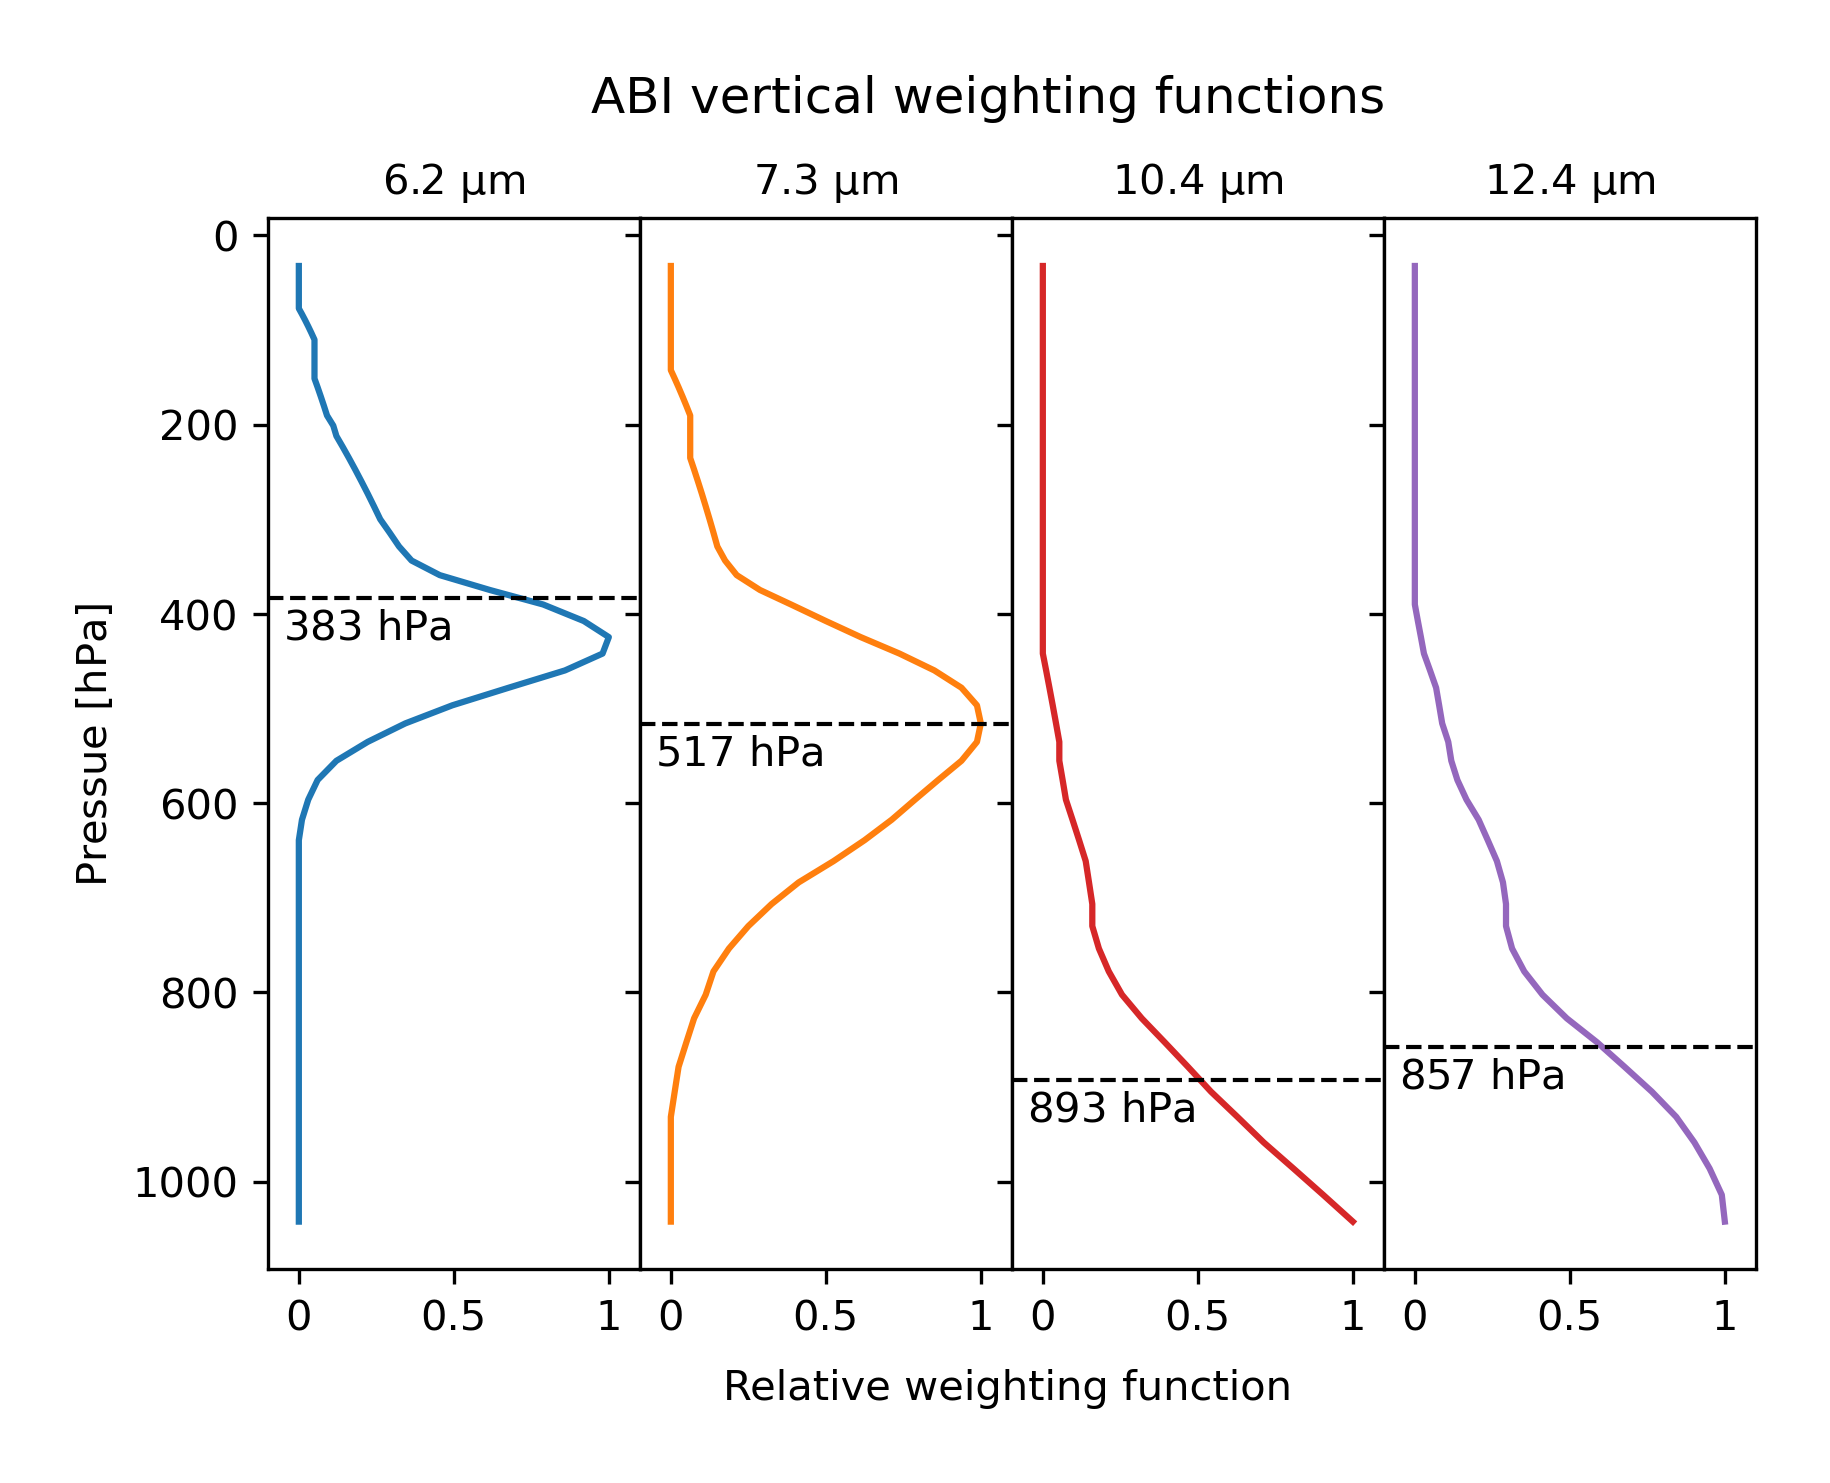
\includegraphics[width=0.9\textwidth]{figures/chapter1_04.png}
    \caption[
    Clear sky vertical weighting functions for the 6.2, 7.3, 10.4 and 12.4\,\unit{\mu m} \acrshort{abi} channels
    ]{
    Clear sky vertical weighting functions for the 6.2, 7.3, 10.4 and 12.4\,\unit{\mu m} \acrshort{abi} channels calculated from rawinsonde profiles measured on 12:00:00 \acrshort{utc} 2020/08/10 at the Tampa RAOB station (KTBW - 72210). The dashed lines and associated pressure values show the weighted average emission height for each channel. Data from {https://cimss.ssec.wisc.edu/goes-wf/plot-viewer/\#/plot-viewer/plot/raob/abi16/default/20200810\_1200Z/72210}
    }
    \label{fig:abi_vertical_weighting}
\end{figure}

The \acrfull{swd}, consisting of the clean \acrshort{ir} window channel minus the dirty \acrshort{ir} window channel (fig.~\ref{fig:abi_channels}\,d), aids in the detection and separation of optically thin anvil cloud (including cirrus outflow) from optically thick anvil due to the difference in ice particle emissivity between these two channels \citep{heidinger_gazing_2009}.
As a result, this combination displays warm temperatures of around 10\,\unit{K} for thin, ice clouds, near 0\,\unit{K} for thick clouds, and approximately 5\,\unit{K} for clear skies due to the contribution of boundary layer \acrshort{wv}.
The \acrshort{swd} is, however, also sensitive to low-level clouds and low-level \acrshort{wv} concentrations, and so cannot be used alone to detect \acrshort{dcc}s.
It remains important to consider the \acrshort{swd} field due to the difficulty in separating anvil clouds from cirrus when using \acrshort{lw} \acrshort{ir} \acrshort{bt} alone \citep{hong_detection_2005}. 
By subtracting the value of the \acrshort{swd} from the \acrshort{wvd}, the sensitivity of the detection scheme to thin cirrus clouds is decreased, reducing the rate of erroneous detections.
Additionally, adding the \acrshort{swd} field to the \acrshort{wvd} field can enhance the appearance of cirrus, enabling the detection of thin ice clouds associated with cirrus outflow and dissipating anvils.

Figure~\ref{fig:abi_vertical_weighting} shows the clear sky vertical weighing functions for the 6.2, 7.3, 10.4 and 12.4\,\unit{\mu m} \acrshort{abi} channels.
The weighting functions are calculated using a radiative transfer model with temperature and humidity profiles observed by rawinsonde observations on 12:00:00 \acrshort{utc} 2020/08/10 at the Tampa RAOB station (KTBW - 72210). 


%t
\begin{table}[tb]
\centering
\begin{tabular}{lrrr}
\tophline
Instrument   & wavelength   & \acrshort{nedt} [300\,K]    & \acrshort{nedt} [220\,K] \\
\middlehline
ABI (GOES--16)         & 6.2\,\unit{\mu m} & 0.013\,K & 0.117\,K\\
             & 7.4\,\unit{\mu m} & 0.024\,K & 0.137\,K\\
             & 10.4\,\unit{\mu m} & 0.028\,K & 0.082\,K\\
             & 12.4\,\unit{\mu m} & 0.023\,K & 0.052\,K\\
\middlehline
SEVIRI (MSG--11)       & 6.2\,\unit{\mu m} & 0.05\,K & 0.45\,K\\
             & 7.3\,\unit{\mu m} & 0.05\,K & 0.29\,K\\
             & 10.8\,\unit{\mu m} & 0.06\,K & 0.17\,K\\
             & 12.0\,\unit{\mu m} & 0.10\,K & 0.24\,K\\
\bottomhline
\end{tabular}
\caption[
Operational \acrshort{nedt} for the \acrshort{abi} and \acrshort{seviri} instruments. 
]{
Operational \acrshort{nedt} for the \acrshort{abi} and \acrshort{seviri} instruments. \acrshort{nedt} is shown both at 300\,K and at 220\,K. \acrshort{abi} data is from {https://www.star.nesdis.noaa.gov/GOESCal/G16\_ABI\_INST\_CAL\_daily\_allmode.php}; \acrshort{seviri} data is from \citet{pili_inorbit_2016}.
} % Table Footnotes
\label{table:channel_nedt}
\end{table}

Measured, on-orbit instrument noise for the \acrshort{abi} and \acrshort{seviri} instruments are provided for each of the four channels selected for use in table~\ref{table:channel_nedt}.
The \acrfull{nedt} values are provided at a reference temperature of 300\,K.
However, as \acrshort{nedt} varies with temperature, it is also important to consider the noise at the colder temperatures typical of anvil clouds.
\acrshort{nedt} at 220\,K were calculated by multiplying the \acrshort{nedt} at 300\,K by the ratio of the partial derivative of the Planck function at 300\,K to that at 220\,K.
This results in a noticeably larger \acrshort{nedt} at the lower temperature, in particular for the \acrshort{wv} channels due to the difference in the gradient of the Planck function between the two temperatures.
Propagating these uncertainties provides estimates of the noise in the \acrshort{wvd} and \acrshort{swd} combinations of 0.180\,K and 0.097\,K respectively for \acrshort{abi}, and 0.54\,K and 0.29\,K for \acrshort{seviri}.

In addition to the \acrshort{nedt}, there are several sources of systematic errors which may affect the observed \acrshort{bt} and channel differences.
Any bias in the \acrshort{abi} and \acrshort{seviri} channels are accounted for in calibration.
Limb darkening at larger satellite zenith angles is harder to account for.
This will have two impacts on the channel differences.
Firstly, it will increase the height at which \acrshort{wv} emissions are observed in the 6.2 and 7.4\,\unit{\mu m} channels, increasing the height at which clouds can be observed.
Secondly, for the \acrshort{swd} combination it may reduce the difference between the two channels, as a higher zenith angle the path length through a cloud layer is longer for the same thickness of cloud, and therefore the difference in temperature will be less between the two channels.

In addition, environmental conditions may affect both the \acrshort{wvd} and \acrshort{swd} combinations.
Changes in humidity may affect the height at which the \acrshort{wvd} is sensitive to clouds, with lower humidity resulting in sensitivity at lower cloud heights.
In addition, the difference between the surface temperature and the cloud temperature will affect the \acrshort{swd}, as the temperature difference is due to a combination of cloud emission and surface emission with a ratio that varies across the two channels.
As a result, if the difference between the cloud and surface temperatures is smaller, so too will be the \acrshort{swd}.
While these biases cannot be removed from the data without retrieving the cloud properties, the choice of methods for cloud detection can limit their impact on the results of detection and tracking.


\subsection{Geostationary Lightning Mapper}

The \acrshort{glm} is also mounted on \acrshort{goes}-16 and detects lightning flashes using an optical transient detector.
The optical transient detector utilises a single, narrow-band \acrshort{nir} channel centred on 777\,\unit{nm} \citep{orville_absolute_1984} to detect momentary changes in brightness associated with lightning events at a frequency of 400\,\unit{\mu s} \citep{christian_global_2003}, providing a 70\,\% minimum efficiency of detection \citep{goodman_goes-r_2013}.
\acrshort{glm} has the same field of view as the \acrshort{abi} instrument, albeit with a lower spatial resolution of 8\,\unit{km} at the sub-satellite point.

As lightning observations are strongly correlated with \acrshort{dcc}s, data from \acrshort{glm} is used to validate the detection of \acrshort{dcc}s using \acrshort{abi}.
The level 2 \acrshort{glm} lightning cluster-filter algorithm product provides a dataset of events, groups and flashes processed from the \acrshort{glm} data \citep{peterson_research_2019}, and filters artifacts from the level 1 \acrshort{glm} data \citep{peterson_removing_2020}.
From this dataset, detected flashes are extracted as evidence of \acrshort{dcc} occurrence.
These locations are then processed by mapping their frequency onto the \acrshort{abi} grid for validation of the algorithm.

\subsection{Next Generation Radar}

\acrshort{nexrad}, also known by its technical name \acrfull{wsr88d}, is a network of weather radars operated by the National Weather Service across the USA \citep{crum_wsr-88d_1993}.
\acrshort{wsr88d} operates in the S-band spectrum, between 2700 and 3000\,\unit{MHz}.
\acrshort{nexrad} stations scan at a range of elevations, typically between 0.5\textdegree\ and 19.5\textdegree\ above horizontal, with a typical scan cycle taking between 4\,\sfrac{1}{2} and 6~minutes, comparable to the temporal sampling of \acrshort{abi} over the \acrshort{conus} region.

Cloud radar reflectivity is proportional to the droplet number density and the droplet radius to the sixth power, making it particularly sensitive to convective rainfall \citep{yau_short_1989}.
As a result, cloud radar observations are ideal for showing the locations of convective cores \citep{austin_relation_1987, rosenfeld_general_1993, zipser_vertical_1994}, and in this chapter it is used to qualitatively assess our ability to detect developing convective cores using \acrshort{abi}.
Level 2 \acrshort{nexrad} radar reflectivity observations from multiple sites are gridded to the same resolution as \acrshort{abi}, and column mean reflectivity is calculated between the altitudes of 2.5 and 15\,\unit{k m}.

\section{Theory} \label{sec:detection_theory}

To better understand how \acrshort{dcc}s appear in \acrshort{goes} \acrshort{abi} observations, a series of experiments were performed using a radiative transfer model.
These experiments were performed using libRadTran v2.0.4 \citep{emde_libradtran_2016}, utilising the DISORT radiative transfer solver \citep{buras_new_2011} and the REPTRAN absorbtion parameterisation \citep{gasteiger_representative_2014}.
The experiments were run using the pyLRT wrapper for libRadTran \citep{gryspeerdt_pylrt_2024}.
A tropical atmospheric profile was used to represent the atmospheric conditions under which deep convection typically occurs.
A list of the options used to set up the radiative transfer model across all simulations is provided in table \ref{table:libradtran}.
All other options have been left as the default settings, including the treatment of relativity humidity which is set to 100\,\% within clouds.

\begin{table}[tb]
\centering
\begin{tabular}{lll}
\tophline
Option          & Value                 & Description                   \\ 
\middlehline
rte\_solver     & disort                & DISORT solver                 \\
source          & thermal               & thermal \acrshort{ir} spectra \\
wavelength      & 3000--15000           & 3--15\,\unit{\mu m}           \\
output\_user    & lambda edir eup uu    & wavelength, direct, diffuse   \\
                &                       &irradiance and all radiances   \\
zout            & 0 TOA                 & surface and \acrshort{toa}    \\
albedo          & 0.5                   & surface albedo                \\
umu             & -1.0, 1.0             & downward \& upward            \\
sza             & 0                     & solar zenith angle            \\
mol\_abs\_param & reptran fine          & REPTRAN parameterisation      \\
atmosphere\_file& afglt.dat             & tropical atmosphere profile   \\
liquid microphysics& Hu                 & \citet{hu_accurate_1993} parameterisation \\
ice microphysics& Fu                    & \citet{fu_accurate_1996} parameterisation \\
\bottomhline
\end{tabular}
\caption[
    Selected options for the libRadTran simulations
    ]{
    Selected options for the libRadTran simulations. All other parameters are left as defaults.
    }
\label{table:libradtran}
\end{table}

In each of the simulations, a cloud layer is included in addition to these options to represent a \acrshort{dcc} in different phases of the lifecycle.
For liquid and ice cloud droplets the Hu parameterisation \citep{hu_accurate_1993} and the Fu scheme \citep{fu_accurate_1996, fu_accurate_1998} are used respectively. 
To show how the simulated clouds are observed by \acrshort{goes}-16, \acrshort{bt} are simulated from the simulated radiances, and then integrated over the spectral response function of each of the \acrshort{abi} channels.

\subsection{Observing growing convective cores}\label{sec:theory_core}

The first experiment aims to represent how a vertically developing \acrshort{dcc} core would appear in \acrshort{abi} observations.
A series of simulations were run with increasing cloud top heights between 1 and 15\,\unit{k m} at 1\,\unit{k m} intervals.
These cloud layers are given a base height of 0\,\unit{k m}, \acrfull{lwc} of 1,000\,\unit{g m^{-2}}, and droplet \acrfull{re} of 15\,\unit{\mu m}.
These values were chosen to represent typical conditions seen in a convective core.
Although liquid droplets are used at all altitudes, simulations with ice cloud droplets showed negligible differences for cloud layers of this thickness.

Figure~\ref{fig:cloud_height_spectra} shows \acrshort{bt} spectra for increasing cloud height, with the spectral response functions of the ten thermal \acrshort{ir} \acrshort{abi} channels plotted in the background.
With such a large \acrshort{lwc}, the \acrshort{bt} matches the \acrshort{ctt} apart from the absorption regions of CO\textsubscript{2} (4.2--4.5\,\unit{\mu m} and \>13.2\,\unit{\mu m}) and ozone (9.4--10.2\,\unit{\mu m}), and the \acrshort{wv} absorption for low-level clouds (5--8\,\unit{\mu m}).


\begin{figure}[tp]
    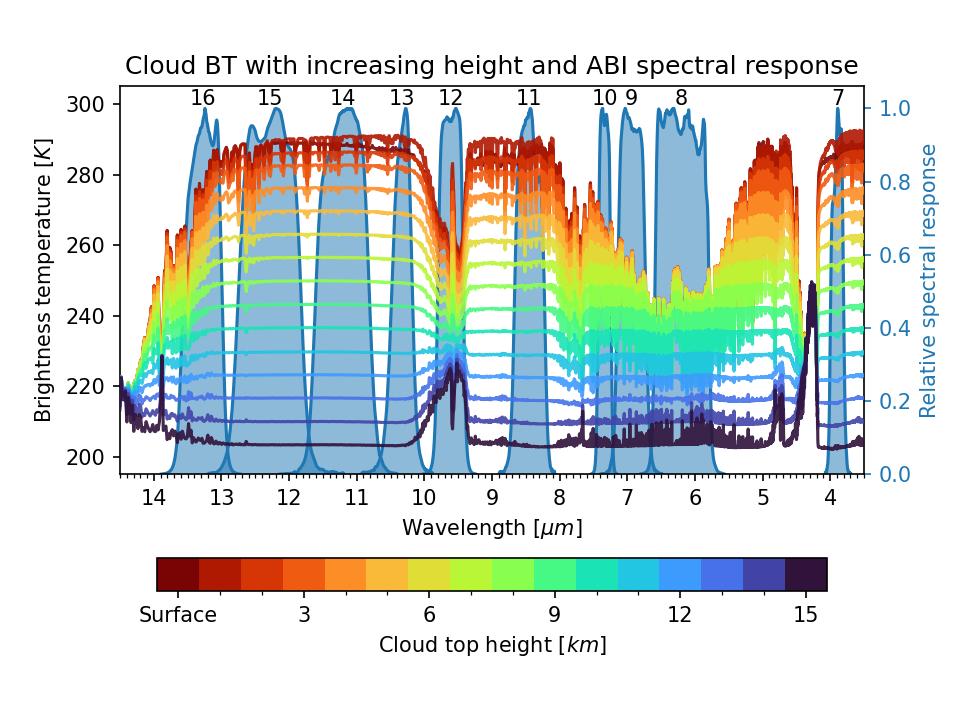
\includegraphics[width=\textwidth]{figures/chapter1_05.png}
    \caption[
    \acrshort{toa} \acrshort{bt} spectra for a simulated cloud representing a \acrshort{dcc} core at heights between 1 and 15\,\unit{k m}
    ]{
    \acrshort{toa} \acrshort{bt} spectra for a simulated cloud representing a \acrshort{dcc} core at heights between 1 and 15\,\unit{k m}, indicating that the largest difference in \acrshort{bt} are seen in the \acrshort{lw} window regions. The filled blue areas in the background show the relative spectral response functions for each of the \acrshort{lw} \acrshort{abi} channels.
    }
    \label{fig:cloud_height_spectra}
\end{figure}


The change in observed \acrshort{bt} with height for the 6.2, 7.3, 10.4, and 12.4\,\unit{\mu m} \acrshort{bt} channels along with the \acrshort{wvd} and \acrshort{swd} is plotted in Fig.~\ref{fig:cloud_height_channels}. 
Above 3\,\unit{k m }, the 10.4 and 12.4\,\unit{\mu m} channels show a constant decrease observed \acrshort{bt} at the moist pseudo-adiabatic lapse rate of 6\,\unit{K}.
Due to the contribution of \acrshort{wv} to the 6.2 and 7.3\,\unit{\mu m} channels at lower \acrfull{cth}, the \acrshort{wvd} shows the most response to vertical development between 6 and 10\,\unit{k m}.
The \acrshort{swd} shows a response to clouds developing at a low altitude.
It has been proposed that this can be used to detect the onset of convection in clear sky conditions before other observations, such as cloud radars \citep{lindsey_use_2014, lindsey_using_2018}.


\begin{figure}[tp]
    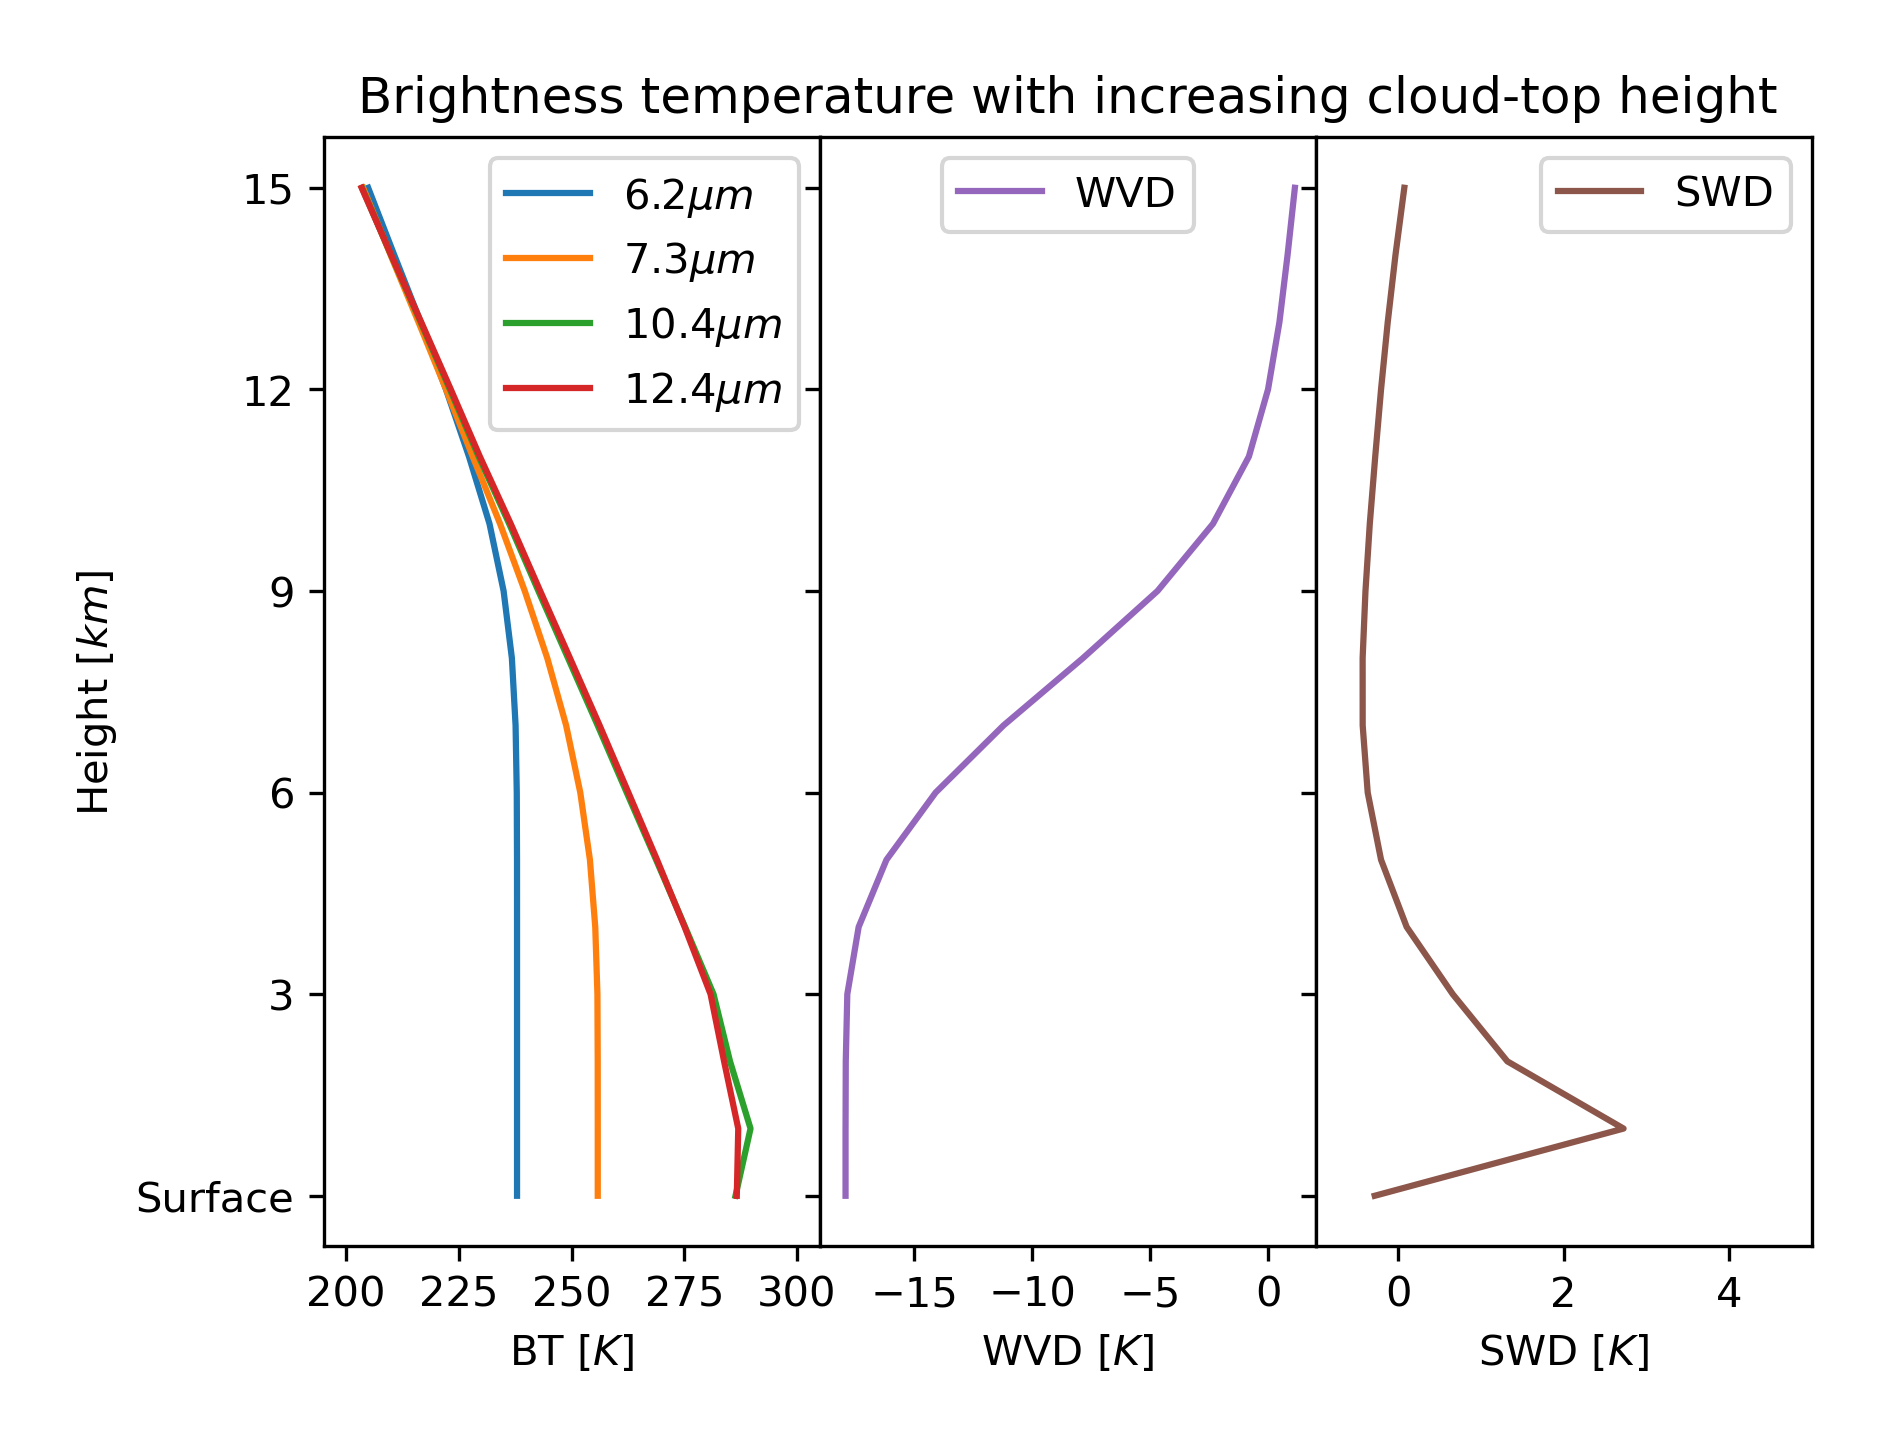
\includegraphics[width=0.9\textwidth]{figures/chapter1_06.png}
    \caption[
    Simulated observations of the 6.2, 7.3, 10.4 and 12.4\,\unit{\mu m} \acrshort{abi} channels, \acrshort{wvd} and \acrshort{swd} for a \acrshort{dcc} core of increasing height
    ]{
    Simulated observations of the 6.2, 7.3, 10.4 and 12.4\,\unit{\mu m} \acrshort{abi} channels, \acrshort{wvd} and \acrshort{swd} for a \acrshort{dcc} core of increasing height.
    }
    \label{fig:cloud_height_channels}
\end{figure}


Figure~\ref{fig:cloud_height_cooling_rates} shows the change of observed \acrshort{bt} in units of K$\cdot\mathrm{minute^{-1}}$ for a convective core rising at a rate of 1\,\unit{ms^{-1}}.
Above 3\,km, the 10.4\,\unit{\mu m} shows a consistent cooling of 0.5\,K$\cdot\mathrm{minute^{-1}}$.
\citet{roberts_nowcasting_2003} found a threshold for severe convection of 8\,\unit{K} cooling over 15~minutes, or approximately 0.5\,K$\cdot\mathrm{minute^{-1}}$, which would represent a cloud top vertical velocity of 1.25\,\unit{m s^{-1}} according to our simulation.
The \acrshort{wvd} shows a maximum rate of change between 7 and 8\,\unit{km}, with a warming rate of half the magnitude of the \acrshort{bt} cooling rate.


\begin{figure}[tp]
    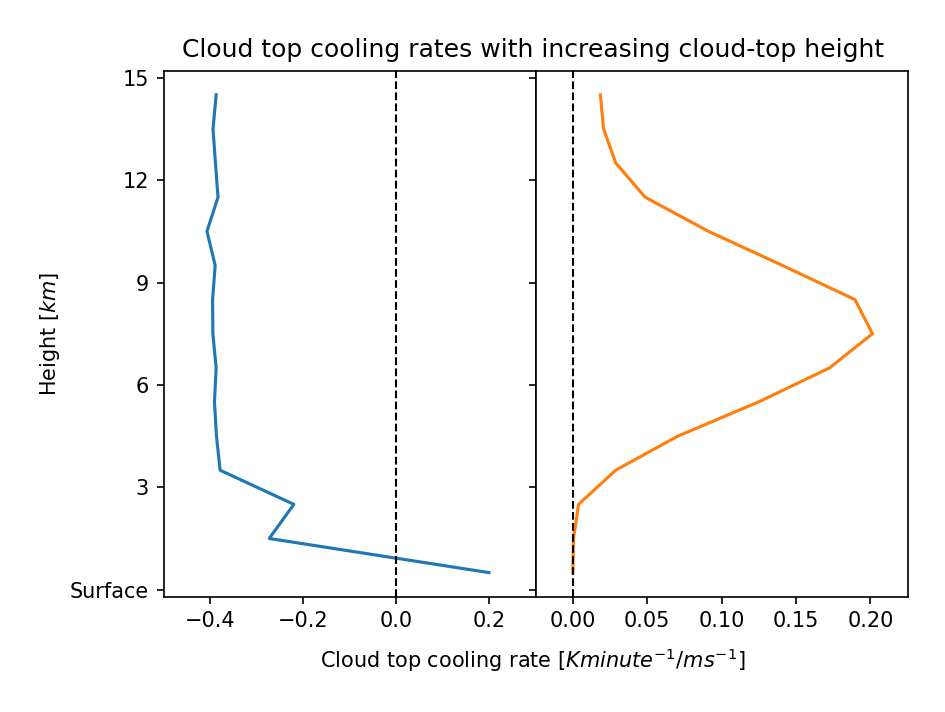
\includegraphics[width=0.9\textwidth]{figures/chapter1_07.png}
    \caption[
    Simulated observed cooling rates of the 10.4\,\unit{\mu m} \acrshort{abi} channels and the \acrshort{wvd} combination for a convective core growing at a rate of 1\,\unit{m s^{-1}}
    ]{
    Simulated observed cooling rates of the 10.4\,\unit{\mu m} \acrshort{abi} channels and the \acrshort{wvd} combination for a convective core growing at a rate of 1\,\unit{m s^{-1}}.
    }
    \label{fig:cloud_height_cooling_rates}
\end{figure}

Using the \acrshort{nedt} values provided in table~\ref{table:channel_nedt}, the uncertainty due to sensor noise in the \acrshort{bt} difference over a five--minute period is approximately 0.047\,K$\cdot \mathrm{minute^{-1}}$, or just less than 10\% of the threshold given by \citet{roberts_nowcasting_2003}.
By averaging the cooling rates over 5 pixels and a 15--minute time period the uncertainty is reduced to 0.012\,K$\cdot \mathrm{minute^{-1}}$, or less than 2.5\%.

Overall, this experiment shows that the 10.4\,\unit{\mu m} \acrshort{bt} channel from \acrshort{abi} can be used to clearly identify a vertically developing core across a wide range of altitudes.
On the other hand, the \acrshort{wvd} is only sensitive to vertically developing clouds in a narrower range of altitudes, and shows a weaker rate of \acrshort{bt} change.
However, this sensitivity to vertical development at a mid to high altitude may help distinguish between \acrshort{dcc}s and other, vertically developed clouds at lower altitudes, such as cumulus congestus.

It should be noted that these simulations were performed with the cloud temperature in equilibrium with the surrounding environment, this is not the case for a convective core which will be warmer than the surrounding air.
Taking 6\,\unit{K/km} as a typical value for the moist pseudo--adiabatic lapse rate, the cooling rate for a convective cloud top rising at 1\,\unit{ms^{-1}} is 0.36\,$\mathrm{K \cdot minute^{-1}}$.
This is similar to the value shown in fig.~\ref{fig:cloud_height_cooling_rates} for the 10.4\,\unit{\mu m} \acrshort{bt}.
In addition, due to the mixing of surrounding air with the convective cloud top, it is expected that the observed temperature profile of the core will be somewhere between that of the environment profile and the moist pseudo--adiabatic lapse rate.
In general, the temperature of the top of convective cores varies very little from the surrounding environment \citep{zipser_cumulonimbus_1980}.

As overshooting tops also cool according to the moist adiabatic lapse rate, the \acrshort{bt} difference method may also detect convective cores that overshoot underlying anvil clouds.
While mixing with the warmer stratospheric air will reduce the cooling rate of the cloud top, the intense convection required to form overshooting tops means that they are still likely to be detected using the same thresholds.
By basing further analysis of convective intensity on the most intense period of the observed cooling rate, the low bias on measurements of convective cores can be reduced.
Detection of overshooting tops may also result in a bias on the number of cores associated with an anvil cloud, as more intense convection may result in detected overshooting tops whereas less intense convection may not be visible above the anvil.
Previous case studies \citep{churchill_development_1984} have shown that the majority of subsequent convection in organised \acrshort{dcc}s tends to occur around the edge of the storm, so it is expected that the masking of developing cores by existing anvil clouds will only have a small impact on the detected number of cores.
In future, research into methods for detecting convective cores under anvil clouds \citep[][e.g.]{apke_relationships_2018} could avoid this bias along with enabling tracking of the full extent of convective core lifetimes.

\subsection{Observing anvil clouds} \label{sec:theory_anvil}

In the second experiment, the appearance of anvil clouds of different \acrfull{od} in \acrshort{abi} observations is investigated.
The simulations were run with an ice cloud with \acrshort{cth} at 14\,\unit{k m}, cloud base height at 12\,\unit{km} and cloud top \acrshort{re} of 20\,\unit{\mu m}, aiming to represent the typical properties of a dissipating anvil cloud \citep{sokol_tropical_2020}.
This simulation was then run for a range of \acrshort{od} between 0.125 and 10, with intervals of 0.125 between 0.125 and 1, 0.25 between 1 and 2, 0.5 between 2 and 5, and 1 between 5 and 10.

\begin{figure}[tp]
    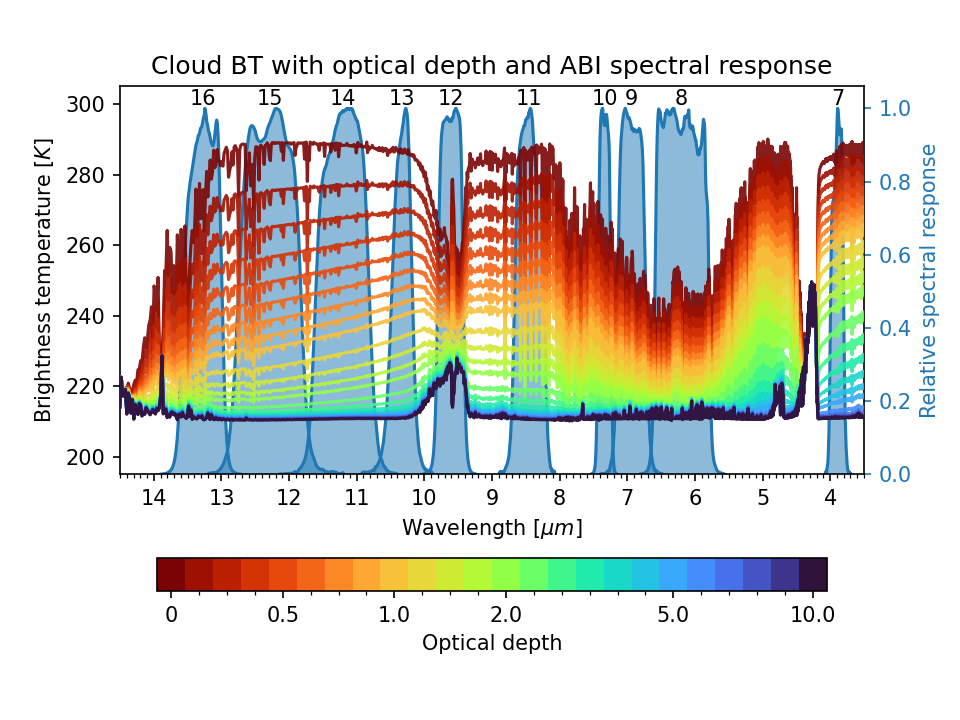
\includegraphics[width=\textwidth]{figures/chapter1_08.png}
    \caption[
    \acrshort{toa} \acrshort{bt} spectra for a simulated anvil cloud with optical thickness between 0 and 10
    ]{
    \acrshort{toa} \acrshort{bt} spectra for a simulated anvil cloud with optical thickness between 0 and 10. 
    }
    \label{fig:optical_depth_spectra}
\end{figure}

\acrshort{bt} spectra for these simulations are shown in Fig.~\ref{fig:optical_depth_spectra}, along with the \acrshort{abi} spectral response functions as in Fig.~\ref{fig:cloud_height_spectra}.
As before, absorption due to CO\textsubscript{2}, ozone, and \acrshort{wv} is seen throughout the spectra.
Unlike the simulations in section \ref{sec:theory_core} however, there is a difference in the \acrshort{bt} spectra across the \acrshort{lw} window (10--13\,\unit{\mu m}) for clouds with \acrshort{od} between 0 and 2, with colder \acrshort{bt} at longer wavelengths.
This is due to the difference in ice emissivity across this range of wavelengths \citep{fu_radiation_2015}.
As the emissivity of ice particles reduces for wavelengths at 10\,\unit{\mu m} and below there is a greater contribution from the atmosphere below the cloud layer and, as a result, warmer \acrshort{bt}s are observed.
It should be noted that this difference is dependent on the size of the ice particles, with smaller \acrshort{re} resulting in a larger difference in emissivity \citep{dubuisson_sensitivity_2008}.


\begin{figure}[tp]
    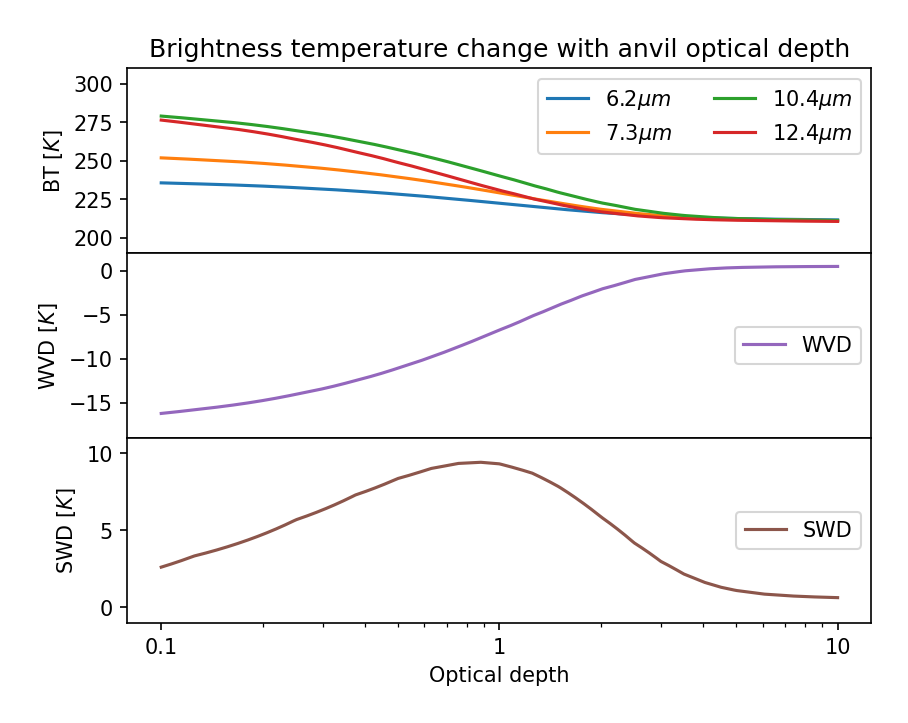
\includegraphics[width=0.9\textwidth]{figures/chapter1_09.png}
    \caption[
    Simulated \acrshort{abi} \acrshort{bt} observations for a \acrshort{dcc} anvil of decreasing optical depth
    ]{
    Simulated \acrshort{abi} \acrshort{bt} observations for a \acrshort{dcc} anvil of decreasing optical depth for the 6.2, 7.3, 10.4, and 12.4\,\unit{\mu m} \acrshort{bt} channels, the \acrshort{wvd} and the \acrshort{swd}.
    }
    \label{fig:optical_depth_channels}
\end{figure}

Figure~\ref{fig:optical_depth_channels} shows simulated \acrshort{abi} observations for the 6.2, 7.3, 10.4, and 12.4\,\unit{\mu m} \acrshort{bt} channels, the \acrshort{wvd} and the \acrshort{swd} for a range of \acrshort{od} between 0.1 and 10.
At high \acrshort{od}, all channels show a cold \acrshort{bt} close to that of the \acrshort{ctt}, however, for \acrshort{od} below 3, the increased contribution from the atmosphere below results in warmer \acrshort{bt}.
The \acrshort{wvd} similarly shows a more negative \acrshort{bt} difference at \acrshort{od} below 3, with a continual decrease for smaller \acrshort{od}.
The \acrshort{swd} however shows an increasingly positive \acrshort{bt} difference for \acrshort{od} below 5, peaking at 10\,\unit{K} around 1~\acrshort{od}.
Below this \acrshort{od} the \acrshort{swd} decreases towards smaller positive values.
As a result, the \acrshort{swd} has the potential to detect thin anvil cirrus at much lower \acrshort{od} than \acrshort{bt} channels or \acrshort{wvd}, down to values around 0.25~\acrfull{od}.

While the \acrshort{bt}, \acrshort{wvd} and \acrshort{swd} are plotted in fig.~\ref{fig:optical_depth_channels} as a function of \acrshort{od} only, other factors may influence the observations.
Changes in cloud height will affect the observed \acrshort{bt}, as higher anvils will have lower temperatures and vice versa.
The \acrshort{wvd} should be unaffected by cloud height as long as the cloud is above heights at which \acrshort{wv} contributes to the vertical weighting functions (fig.~\ref{fig:abi_vertical_weighting}), and above 12\,km there is little change with height (fig.~\ref{fig:cloud_height_cooling_rates}). 
Changes in tropospheric humidity will affect the \acrshort{wvd} as this will change the height of the weighting function response and hence the height at which the \acrshort{wvd} is sensitive to clouds.
As the majority of \acrshort{dcc}s are expected to occur in relatively humid environments it is expected that this effect will be minimal.
However, in particularly cold, dry conditions this may result in lower level clouds being erroneously detected as anvils.
Finally, the \acrshort{swd} has some sensitivity to \acrshort{re}, as larger particles show a smaller difference in emissivity between 10 and 12\,\unit{\mu m}.
The effect of this is small, and the peak \acrshort{swd} remains present at the same optical depth.


\section{Method} \label{sec:tracking_method}

In this section, a novel method for detecting and tracking both the growing cores and anvils clouds of \acrshort{dcc}s, consisting of the following steps:

\begin{enumerate}
    \item Ingest of \acrshort{lw} \acrshort{ir} \acrshort{bt} fields from geostationary satellite imagery, including calculation of \acrshort{wvd} and \acrshort{swd} fields from \acrshort{ir} \acrshort{wv} and \acrshort{lw} \acrshort{ir} window channels.
    \item Calculation of optical flow vectors to be used as an \textit{a priori} estimate of cloud motion for use in the semi-lagrangian framework.
    \item Detection of growing \acrshort{dcc} cores using cloud top cooling rate.
    \item Detection of thick and thin anvil clouds associated with detected cores using a semi-lagrangian "3D" watershedding method. 
    \item Grouping of cores into multi-core systems, calculation of statistics and validation using lightning observations.
\end{enumerate}



\subsection{Estimation of cloud motion vectors using optical flow} \label{sec:optical_flow}

The retrieval of \acrshort{amv}s has been performed since the earliest geostationary satellite observations \citep{menzel_cloud_2001}.
\acrshort{amv}s provide information about the motion of clouds in the atmosphere, including \acrshort{dcc}s \citep{bedka_application_2005}, and are routinely generated for the majority of operational geostationary earth observation satellites, including \acrshort{goes}-16 \citep{daniels_algorithm_nodate}. 
However, although \acrshort{amv}s may provide useful information about the motion of \acrshort{dcc}s, the non-geostrophic nature of wind fields in these conditions may result in the \acrshort{amv}s being calculated inaccurately or rejected by quality control checks \citep{bedka_application_2005}.

Optical flow algorithms are a family of algorithms used to estimate the apparent motion of objects observed in a series of images \citep{aggarwal_computation_1988}. 
A wide range of optical flow algorithms exist, and these have been successfully applied to many computer vision applications. 
It should be noted that optical flow does not necessarily represent the physical motion of an object, but is instead an estimation of the relative motion between an object and the observer and additionally any change in the apparent object (including growing, shrinking or other warping of the object). 

Optical flow algorithms have been previously shown to be accurate for the prediction of \acrshort{amv}s using geostationary satellite images \citep{wu_deriving_2016}, as long as the observations are sufficiently frequent such that the motion of unique features between images is less than the length scale at which neighbouring features can be resolved \citep{bresky_feasibility_2006}.
\citet{heikenfeld_tobac_2019} found that at imaging frequencies of less than 5~minutes the motion of \acrshort{dcc} cores was less than the spacing between neighbouring cores in the majority of cases, indicating that the frequency of the \acrshort{abi} \acrshort{conus} scan region is suitable for calculating optical flow vectors of \acrshort{dcc}s.
The use of optical flow has several advantages over traditional \acrshort{amv}s for the retrieval of \acrshort{dcc} motion vectors: optical flow can be calculated quickly using only two subsequent images and no \textit{a priori} information, aiding in near real-time applications; and also have no requirement for geostrophic balance. 
Optical flow algorithms are routinely used in the nowcasting of convective precipitation, and can be used to provide accurate predictions of \acrshort{dcc} with an hour of lead time using either radar or satellite observations \citep[e.g.][]{bowler_development_2004, bechini_enhanced_2017, woo_operational_2017}.
Optical flow, and similar motion vector techniques, have also been successfully applied to both the detection of developing deep convection \citep{zinner_cb-tram_2008, zhang_locating_2014} and tracking detected deep convective features \citep{senf_size-resolved_2018} separately.

It should be noted that optical flow is used to estimate the apparent motion of the cloud field between subsequent images, with the aim of using these vectors to map the locations of \acrshort{dcc}s from one step to the next, instead of calculating actual \acrshort{amv}s corresponding to winds.
This approach avoids a number of challenges with the use of optical flow for calculating \acrshort{amv}s including the estimation of the height of estimated flow vectors and the detection of diverging or converging motion vector fields in situations of growing and dissipating clouds respectively.
In the latter case, both divergence and convergence within the optical flow vector field are intentionally included to map both the location and shape of observed clouds between time steps.

\subsubsection{Evaluation of Optical Flow Methods}

As different optical flow algorithms may provide better accuracy in different situations \citep{baker_database_2011}, several algorithms are compared to assess their suitability for tracking the motions of \acrshort{dcc}s.
Six different optical flow algorithms, implemented in the OpenCV library \citep{opencv_library}, are considered, which are listed below:

\begin{itemize}
    \item Farnebäck \citep{farneback_two-frame_2003}
    \item \acrfull{dis} \citep{kroeger_fast_2016}
    \item DeepFlow \citep{weinzaepfel_deepflow_2013}
    \item \acrfull{dualtvl1} \citep{zach_duality_2007, perez_tv-l1_2013}
    \item Sparse to Dense \citep{bouguet_pyramidal_1999}
    \item \acrfull{pca}-Flow \citep{wulff_efficient_2015}
\end{itemize}

The first four of these algorithms are dense optical flow methods, which calculate motion vectors for every pixel in the image.
The final two calculate sparse optical flow---motion vectors between detected objects in each image, rather than individual pixels---and then map these to all pixels based on a region segmentation approach.
The sparse to dense and \acrshort{pca}-flow algorithms use the Lucas-Kanade method \citep{lucas_iterative_1981} and the \acrshort{pca} method respectively to calculate the sparse motion vectors.

Each algorithm was applied to a sequence of images from the 10.4\,\unit{\mu m} channel, with the algorithms estimating motion vectors between each consecutive pair of images.
As the methods require 8-bit images, a linear normalisation was applied to the \acrshort{bt} images between each pair's minimum and maximum values.
To improve the accuracy of the detected motion vectors, a variational refinement process \citep{brox_high_2004} is applied to the calculated flow vectors.
This process minimises the energy functional of the pixel value, pixel gradient, and local smoothness to reduce the angular error of the detected flow vectors.
Finally, vectors are calculated both forwards and backward in time between each pair of images, and these two sets of vectors are interpolated to each other's locations and averaged to ensure that they are equal and opposite.

Figure~\ref{fig:opt_flow_comparison} shows the \acrshort{abi} \acrshort{bt} at 19:00:00~\acrshort{utc} (fig.~\ref{fig:opt_flow_comparison}\,a), along with the optical flow vectors calculated by each of the algorithms with the subsequent time step.
For each set of optical flow vectors, the average vector over each 5\texttimes 5-pixel area is plotted by the red arrows, and the vector velocity magnitude is plotted in the background.
The two sparse methods (fig.~\ref{fig:opt_flow_comparison}\,f,g) show a closer match of the areas where optical flow vectors to the edge of the anvil cloud than the dense methods (fig.~\ref{fig:opt_flow_comparison}\,b--e), which have a tendency to smooth the detected vectors over a large area.
Of all the methods, the Farnebäck algorithm tends to produce larger magnitudes, but correctly detects zero flow in areas without clouds, unlike most of the other algorithms.


\begin{figure}[tp]
    \centering
    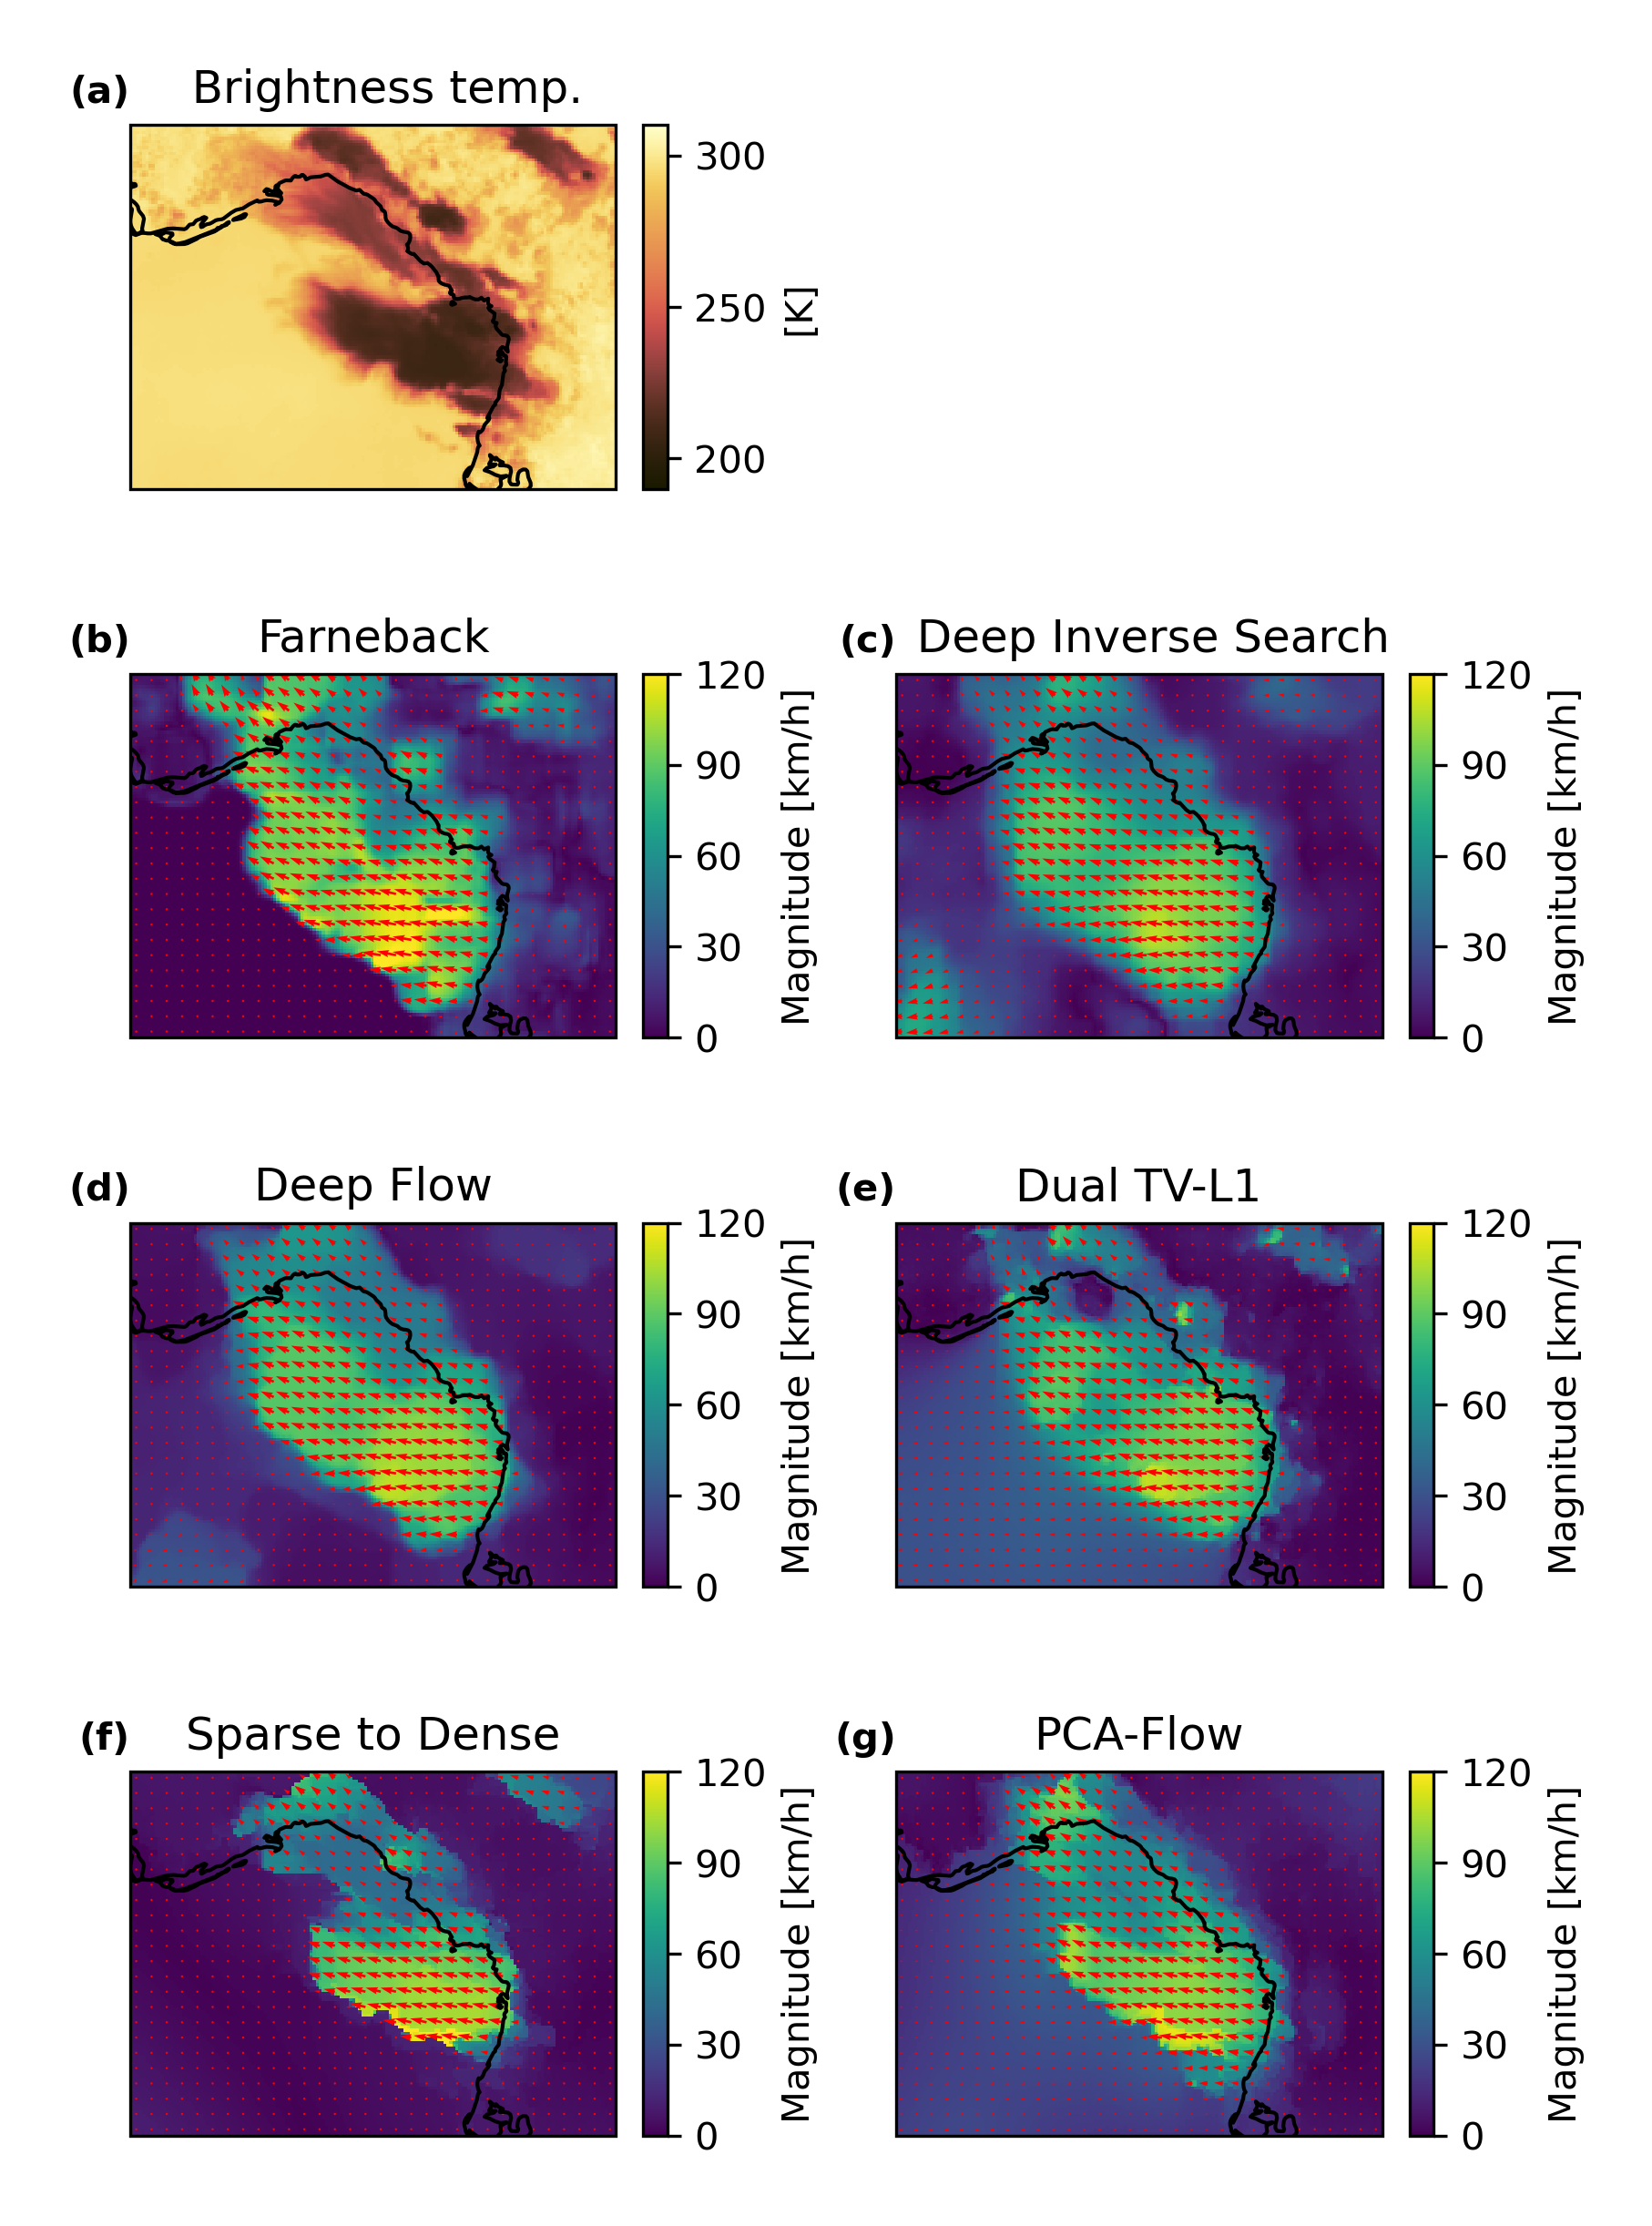
\includegraphics[width=0.9\textwidth]{figures/chapter1_10.png}
    \caption[
    A comparison of the motion vector fields generated by different optical flow methods
    ]{
    A comparison of the motion vector fields generated by the (b) Farnebäck, (c) \acrshort{dis}, (d) DeepFlow, (e) \acrshort{dualtvl1}, (f) Sparse to Dense, and (g) \acrshort{pca}-Flow. Optical flow vectors shown are estimated between the 10.4\,\unit{\mu m} channel at 19:00:00 \acrshort{utc} (a) and the subsequent image. Red arrows (b--g) show the motion vectors averaged over each 5\texttimes 5-pixel area is plotted by the red arrows, and the background shows the magnitude of the velocity vectors.
    }
    \label{fig:opt_flow_comparison}
\end{figure}


Figure~\ref{fig:opt_flow_differences} shows the difference in \acrshort{bt} between subsequent observations when taking into account the cloud motion predicted by the different optical flow algorithms.
The plots are again shown for the time step at 19:00:00~\acrshort{utc}, with the 10.4\,\unit{\mu m} \acrshort{bt} at this time step shown again for reference in fig.~\ref{fig:opt_flow_differences}\,a.
Figure~\ref{fig:opt_flow_differences}\,b shows the Eulerian difference in \acrshort{bt}; the difference in the \acrshort{bt} observed at the same pixel locations on subsequent time steps.
Large cooling rates are seen of the left (downwind) side of the anvil cloud, not because the \acrshort{ctt} is cooling, but because of the expansion of the anvil cloud into previously cloud-free areas.
Separating these observations of cooling \acrshort{bt} caused by the motion and expansion of the anvil cloud from those due to the vertical growth of the \acrshort{dcc} is the main objective of the semi-Lagrangian approach.


\begin{figure}[tp]
    \centering
    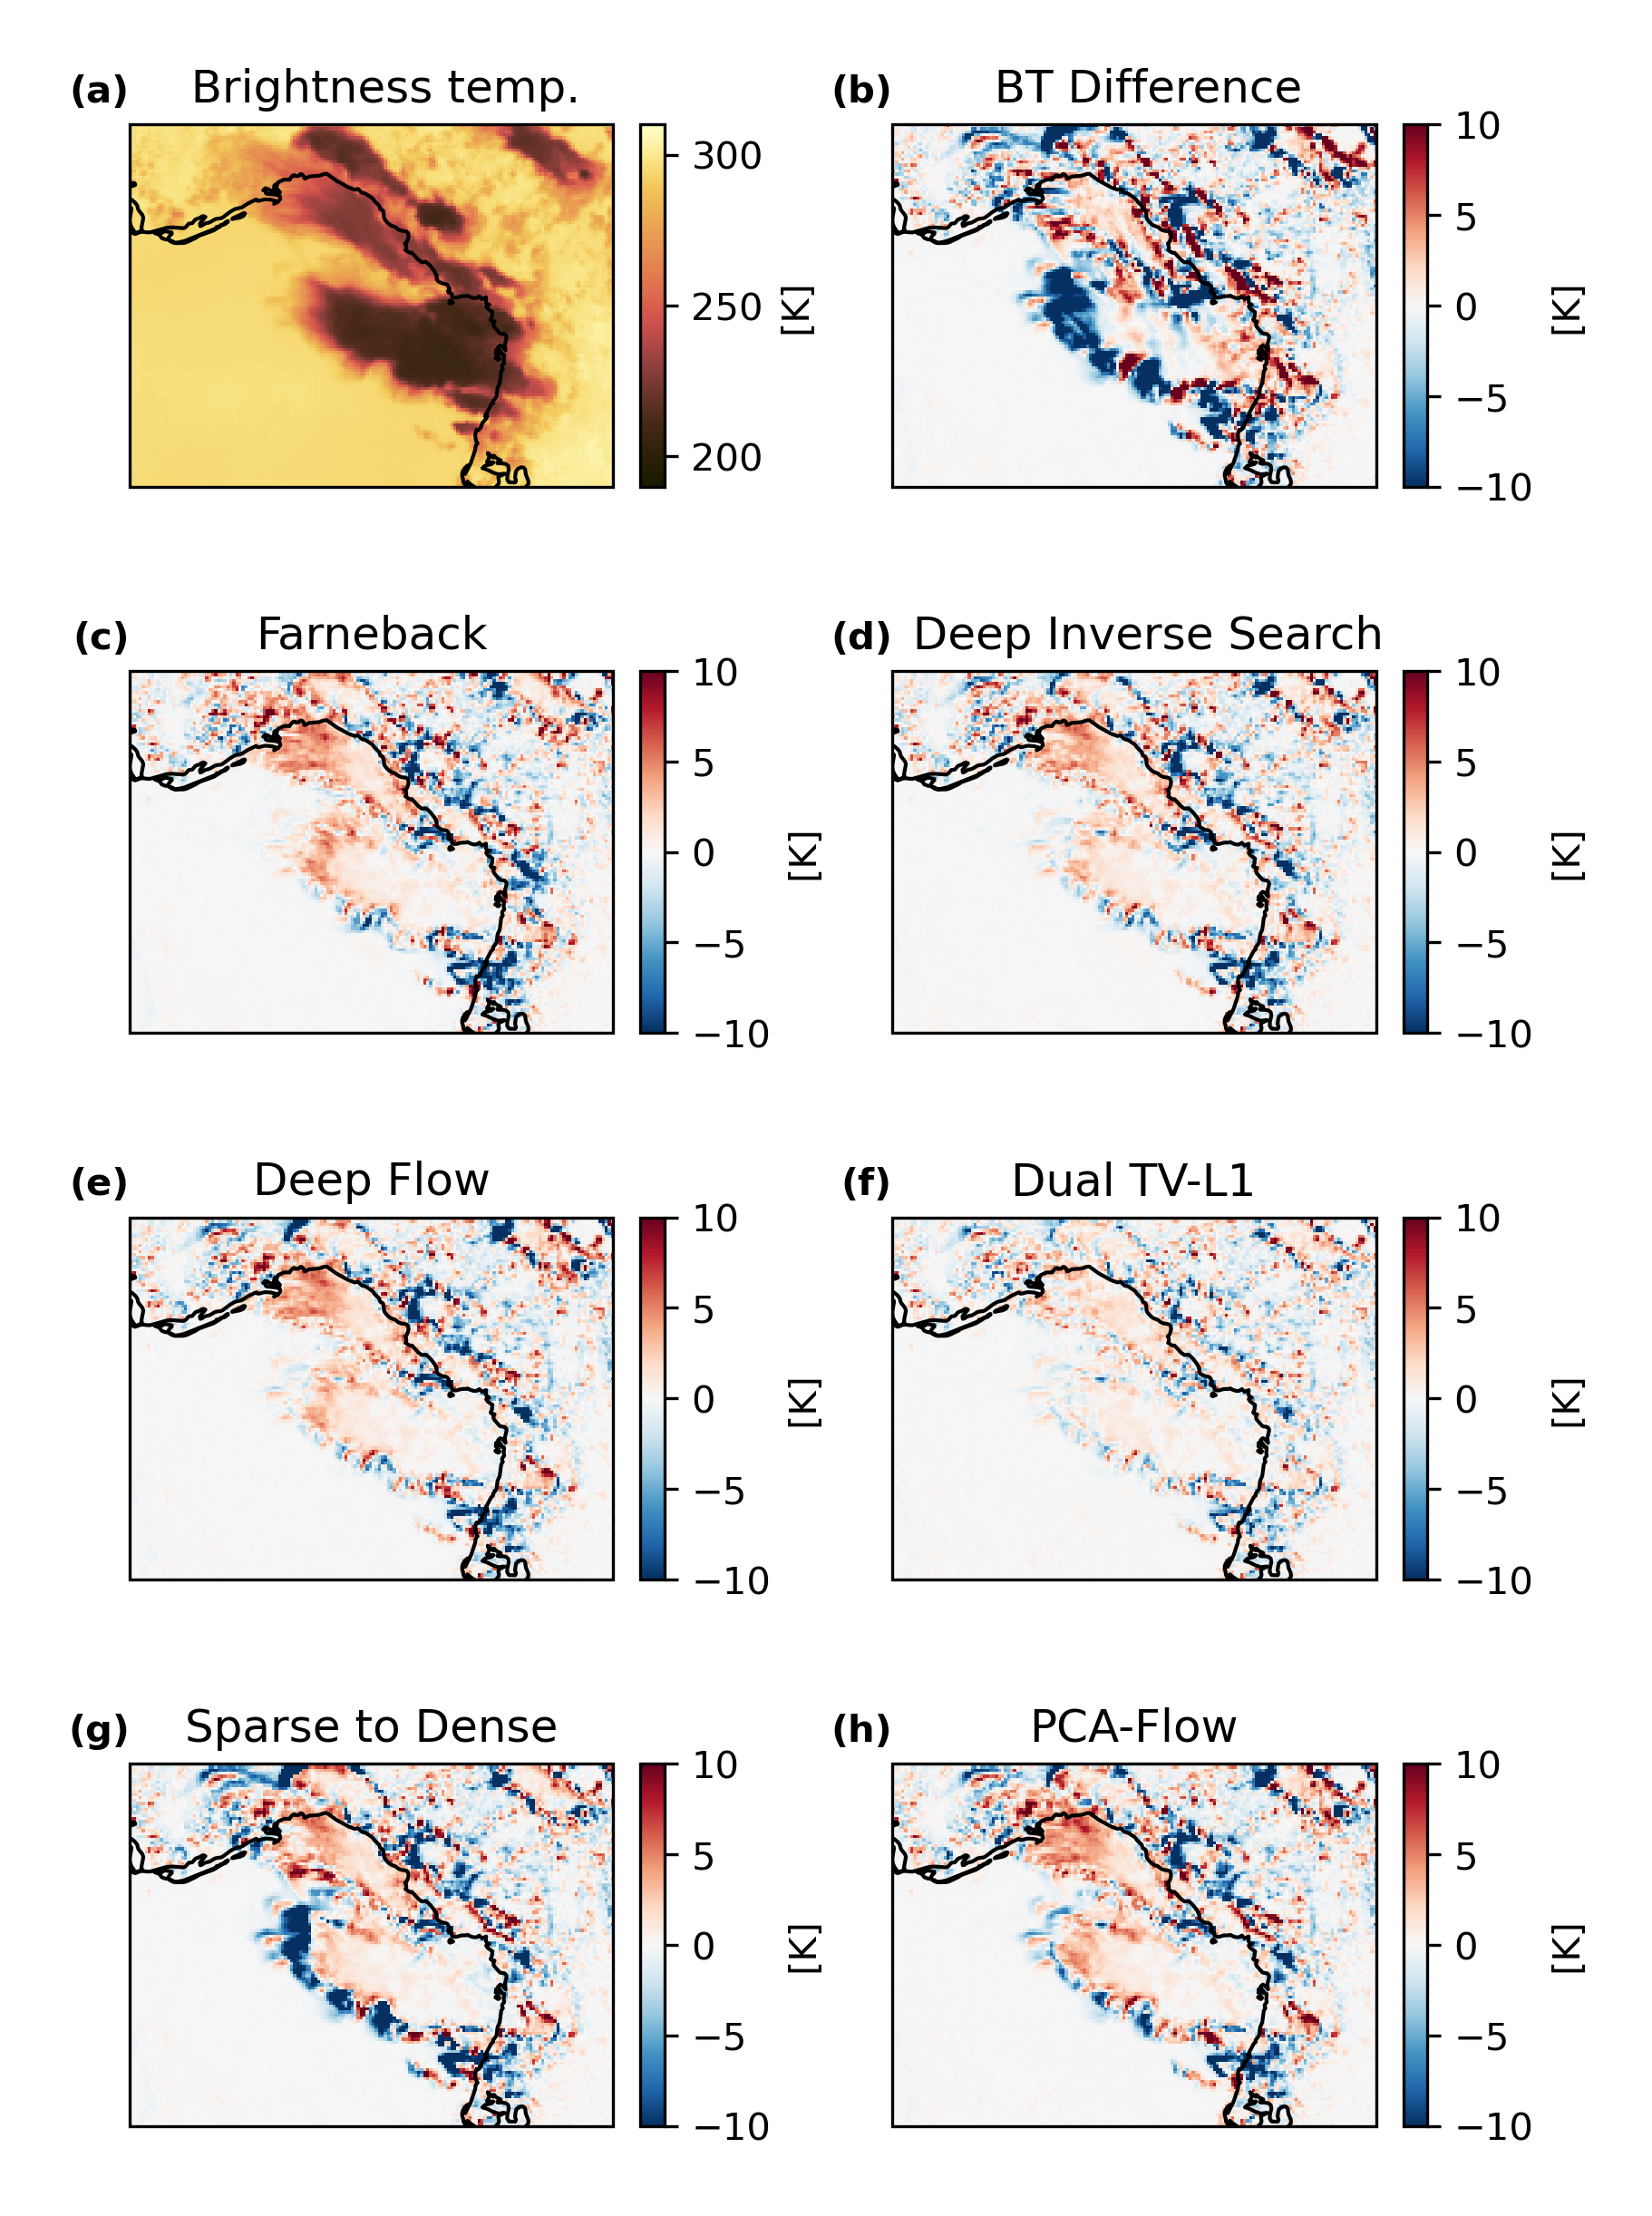
\includegraphics[width=0.9\textwidth]{figures/chapter1_11.png}
    \caption[
    The difference in \acrshort{bt} between subsequent \acrshort{abi} observations when taking into account the cloud motion predicted by the different optical flow algorithms.
    ]{
    The difference in \acrshort{bt} between subsequent \acrshort{abi} observations when taking into account the cloud motion predicted by the different optical flow algorithms. The plots are again shown for the time step at 19:00:00~\acrshort{utc}, with the 10.4\,\unit{\mu m} \acrshort{bt} at this time step shown for reference (a). b: the difference in \acrshort{bt} without accounting for cloud motion; c--h: the Lagrangian difference in \acrshort{bt} using motion vectors predicted by each of the optical flow algorithms.
    }
    \label{fig:opt_flow_differences}
\end{figure}


The dense optical flow methods (fig.~\ref{fig:opt_flow_differences}\,c--f) show good performance in removing the anomalous cooling observations seen downwind of the anvil cloud.
The Farnebäck, \acrshort{dis} and DeepFlow algorithms (fig.~\ref{fig:opt_flow_differences}\,c--e) all show a warming tendency towards the edge of the anvil cloud.
Although this may be explained by an overestimation of the cloud motion by these algorithms, this may also be a real observation of apparent warming due to thinning of the detraining anvil cloud.
The \acrshort{dualtvl1} algorithm (fig.~\ref{fig:opt_flow_differences}\,f) shows generally smaller differences than the other algorithms.
This is likely due to the algorithm accounting for changes in brightness between observations, whereas the other algorithms assume that the brightness of tracked objects remains constant between observations.

The two sparse optical flow algorithms (fig.~\ref{fig:opt_flow_differences}\,g,h) both show worse performance, with the sparse to dense method performing particularly poorly.
Both algorithms show cooling downwind of the anvil, likely because the region-based methods used to map the sparse motion vectors to the whole image do not detect this region well.

\begin{figure}[tp]
    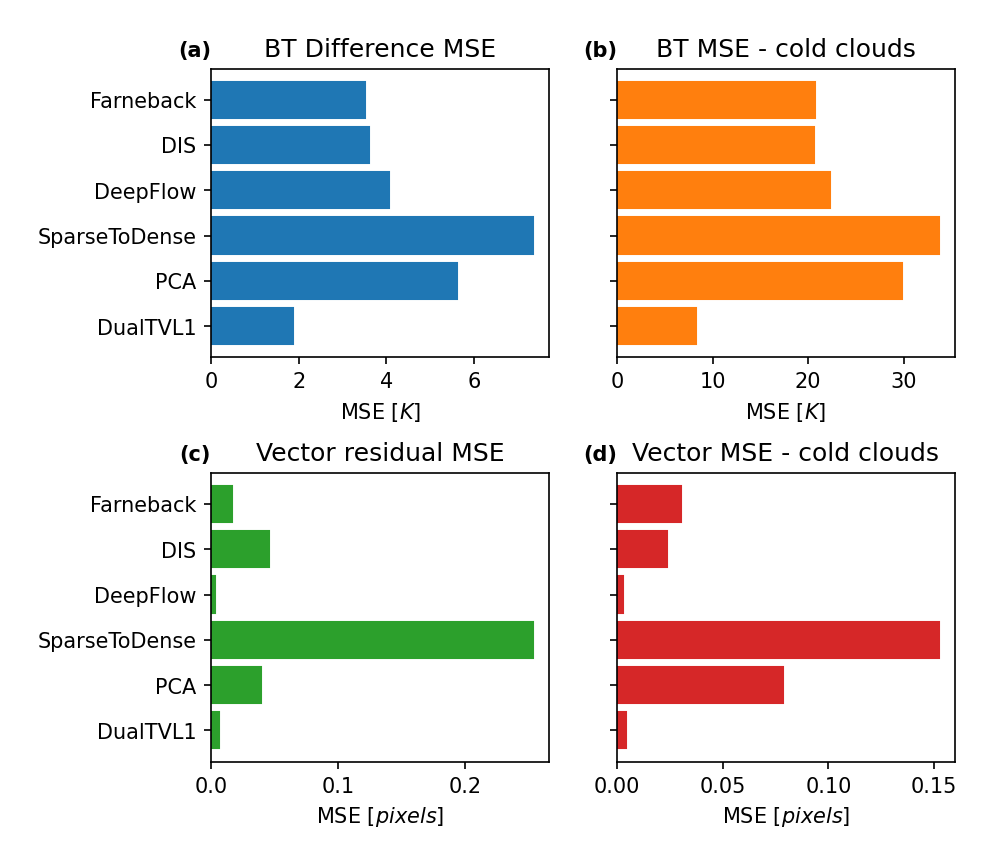
\includegraphics[width=0.9\textwidth]{figures/chapter1_12.png}
    \caption[
    A comparison of the \acrshort{bt} difference and residual vector magnitude \acrshort{rmse} for each of the optical flow algorithms
    ]{
    A comparison of the \acrshort{rmse} for each of the optical flow algorithms. a: \acrshort{bt} difference \acrshort{rmse} for all pixels and (b) for pixels with \acrshort{bt} $<$ 273\,\unit{K}. c: \acrshort{rmse} of the residual vector magnitude for all pixels and (d) for pixels with \acrshort{bt} $<$ 273\,\unit{K}.
    }
    \label{fig:opt_flow_mse}
\end{figure}

Figure~\ref{fig:opt_flow_mse}\,a shows the \acrfull{rmse} of the \acrshort{bt} differences shown in fig.~\ref{fig:opt_flow_differences} for each algorithm.
As seen in fig.~\ref{fig:opt_flow_differences}, the \acrshort{dualtvl1} algorithm has the smallest differences, the other dense algorithms perform similarly, and the \acrshort{pca}-Flow and sparse to dense algorithms perform the worst.
Some differences in the \acrshort{bt} should be expected due to actual changes in the \acrshort{ctt}.
Figure~\ref{fig:opt_flow_mse}\,b shows the \acrshort{rmse} of the \acrshort{bt} differences for pixels with \acrshort{bt} less than 273\,\unit{K}, representing cold cloud observations.
While the \acrshort{rmse} shown here for all algorithms is large compared to the sensor noise previously calculated for the \acrshort{bt} difference in section~\ref{sec:theory_core} (0.47\,K), it should be noted that some of the \acrshort{rmse} here is due to contributions from changes in the height of the anvil cloud.
As a result, the actual error in the \acrshort{bt} difference over time due to horizontal cloud motions not captured by the optical flow algorithm is likely much smaller, on a similar magnitude to the \acrshort{nedt}.

To estimate the uncertainty in the calculated motion vectors, the residual motion vectors are calculated for each algorithm.
The residual motion is calculated by first warping each image to the locations predicted by the optical flow vectors, in the same manner used to calculate the \acrshort{bt} differences in fig.~\ref{fig:opt_flow_differences}.
Then the optical flow algorithms are used to calculate a second set of residual vectors between each image and the subsequent warped image.
In theory, if the initial motion vectors were calculated perfectly, warping the image by the optical flow vectors should result in the subsequent cloud in the same position as the prior image, and so the second set of motion vectors should calculate as zero.
The magnitude of the residual motion vectors is therefore considered as the uncertainty in the initial set of motion vectors.

Figure~\ref{fig:opt_flow_mse}\,c,d show the \acrshort{rmse} of the residual vector magnitudes for all pixels and pixels less than 273\,\unit{K} respectively.
The DeepFlow and \acrshort{dualtvl1} algorithms again show the best accuracy, and sparse to dense the worst.
The Farnebäck algorithm shows good accuracy across all pixels, as seen in the ability to correctly detect zero motion in cloudless skies in fig.~\ref{fig:opt_flow_comparison}.
However, when considering only cold pixels the Farnebäck algorithm performs slightly worse than \acrshort{dis}.

The results shown in fig.~\ref{fig:opt_flow_mse} suggest that the \acrshort{dualtvl1} algorithm is the best choice for estimating the motion vectors in satellite observations of \acrshort{dcc}.
However, due to the large size and long sequences of images produced by \acrshort{abi}, it is also important to consider the computational cost of each algorithm.
Figure~\ref{fig:opt_flow_cost} shows the run time in seconds for each algorithm applied to a sequence of 48 300\texttimes300~pixel \acrshort{abi} \acrshort{bt} images.
Both the DeepFlow and \acrshort{dualtvl1} algorithms show significantly longer run times than any of the other algorithms.
As a result, the Farnebäck algorithm has been selected for the tracking method as it offers the best balance of accuracy and computational performance for running on large datasets.


\begin{figure}[tp]
    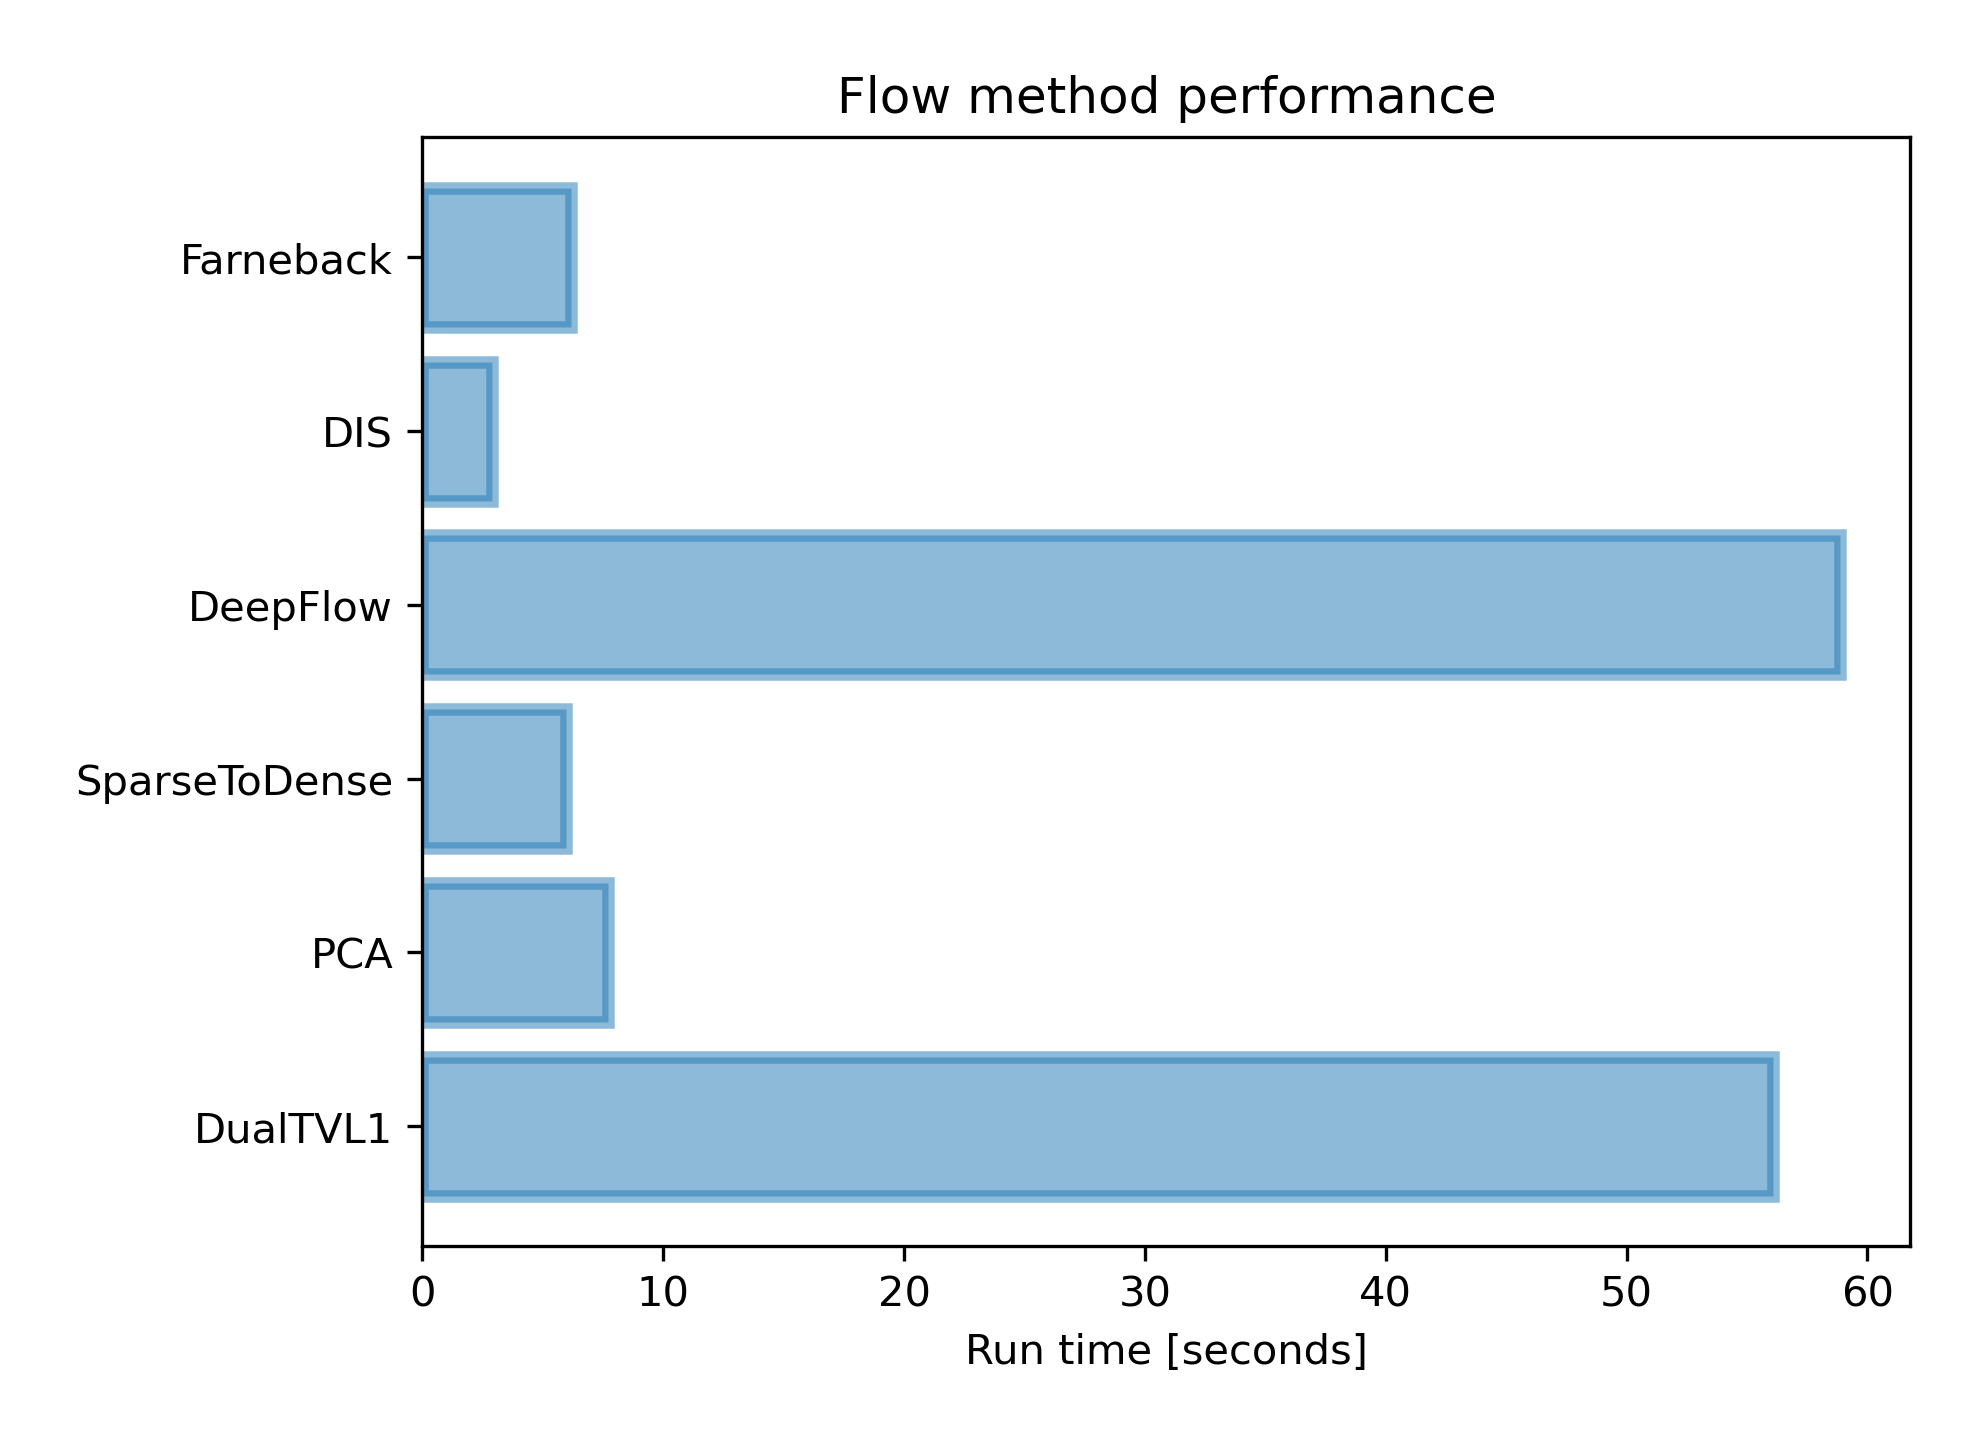
\includegraphics[width=0.9\textwidth]{figures/chapter1_13.png}
    \caption[
    A comparison of the computational performance of each optical flow method
    ]{
    A comparison of the computational performance of each optical flow method. Run-time was measured for a sequence of 48 300\texttimes300 pixel \acrshort{abi} 10.4\,\unit{\mu m} \acrshort{bt} images.
    }
    \label{fig:opt_flow_cost}
\end{figure}


An example of the motion vectors calculated by the Farnebäck algorithm when applied to the 10.4\,\unit{\mu m} \acrshort{bt} field is shown in fig.~\ref{fig:optical_flow}.
Figure~\ref{fig:optical_flow}\,c shows the residual flow vectors, which are small compared to the detected cloud motion vectors (fig.~\ref{fig:optical_flow}\,b).
The main areas in which residual flow vectors can be seen are the regions around the edge of anvil clouds and in the centre of thick anvil clouds where there are no clear features to track.
Figure~\ref{fig:optical_flow}\,d shows the distribution of residual vector errors proportional to the detected cloud motion vectors.
The majority of the residual errors are close to zero, and very few exceed 0.5.
As, in the majority of applications for the semi-Lagrangian framework, only the motion rounded to the nearest pixel is of interest, these errors are considered acceptable.


%f
\begin{figure}[tp]
    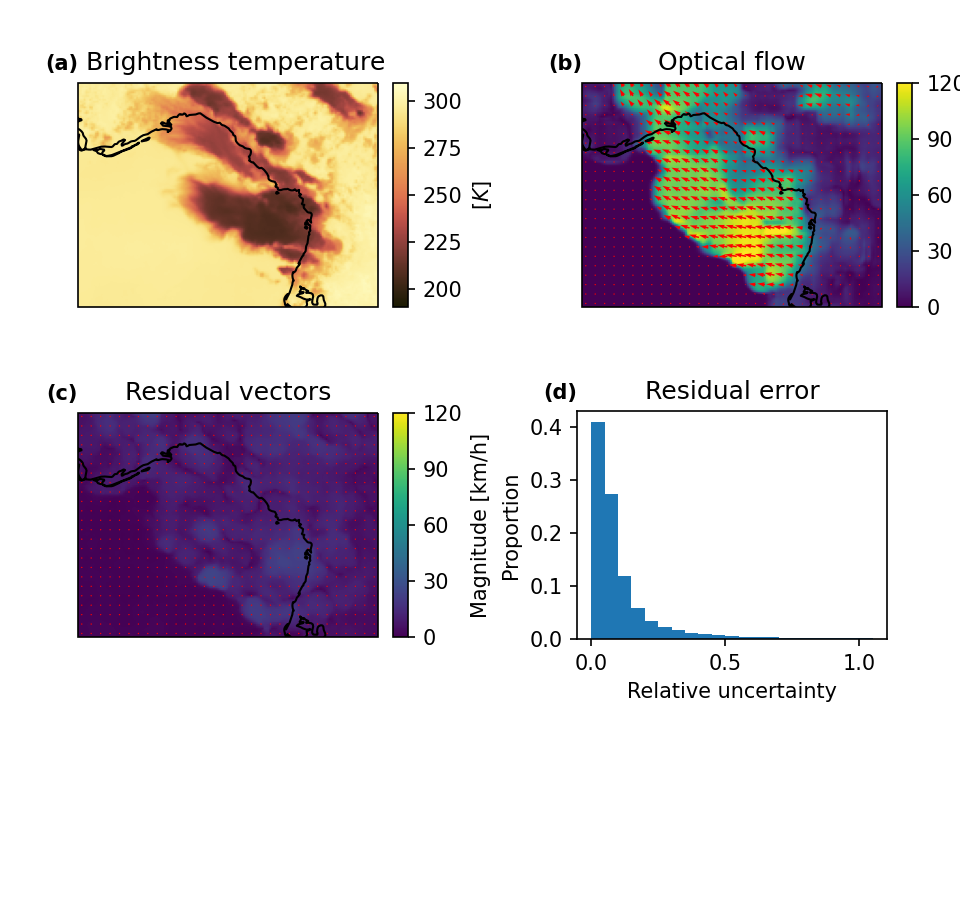
\includegraphics[width=\textwidth]{figures/chapter1_14.png}
    \caption[
    An example of the motion vectors and their residual errors calculated using the Farnebäck algorithm
    ]{
    An example of the motion vectors and their residual errors calculated using the Farnebäck algorithm. a: the 10.4\,\unit{\mu m} \acrshort{bt} field at 19:00:00~\acrshort{utc} for which the motion vectors are shown. b: the calculated motion vectors. c: the residual motion vectors, indicating the uncertainty in the optical flow. d: the magnitude of the residual motion vectors as a proportion of the magnitude of the optical flow vectors for cold pixels (less than 273\,\unit{K})
    }
    \label{fig:optical_flow}
\end{figure}


Two potential sources of uncertainty are the assumptions made by the Farnebäck algorithm that the feature being tracked remains the same size and intensity in subsequent images.
For optical flow tracking using \acrshort{bt} images of growing \acrshort{dcc}s, neither of these assumptions are true.
However, steps have been taken to reduce the impact of both these sources of uncertainty on the tracking algorithm.
For the first of these assumptions, it is found that in the case of small, fast-moving \acrshort{dcc}s---where the accuracy of the optical flow vectors is most important---the changes in the size of the \acrshort{dcc} is small compared to the overall motion, and so the uncertainty introduced is small.
Comparably, for large \acrshort{dcc}s where the changes in size may be large compared to the motion, the uncertainty has less impact on the tracking algorithm.
In the worst-case scenario, the estimated optical flow field will be zero, in which case the "3D" detection and tracking algorithm works in the same manner as that of \citet{fiolleau_algorithm_2013}, which is suitable for use on these larger \acrshort{dcc}s.

\subsection{A Semi-Lagrangian Framework for Morphological Image Processing}

Morphological image operations analyse images using their geometrical and structural properties.
Core to many morphological algorithms, from simple filters to complex neural networks \citep{kalchbrenner_convolutional_2014}, is the kernel, or convolution method.
A convolution method performs operations on the pixels of an image by applying a convolution stencil to the pixel and its neighbours.
In a conventional convolution scheme, such as that used in the methods of \citet{fiolleau_algorithm_2013}, the convolution stencil acts on adjacent pixels in both time and space (see fig.~\ref{fig:convolution_kernels}\,a).
In this Eulerian framework, different locations in time are considered in the same manner as those in the spatial dimensions.
However, previous analysis of \acrshort{dcc}s has shown that the motion of convective cores between images can be similar to the spacing of cores and their size \citep{heikenfeld_tobac_2019}.
As a result, it is important to include the effects of advection when comparing images across time steps.


%f
\begin{figure}[tp]
    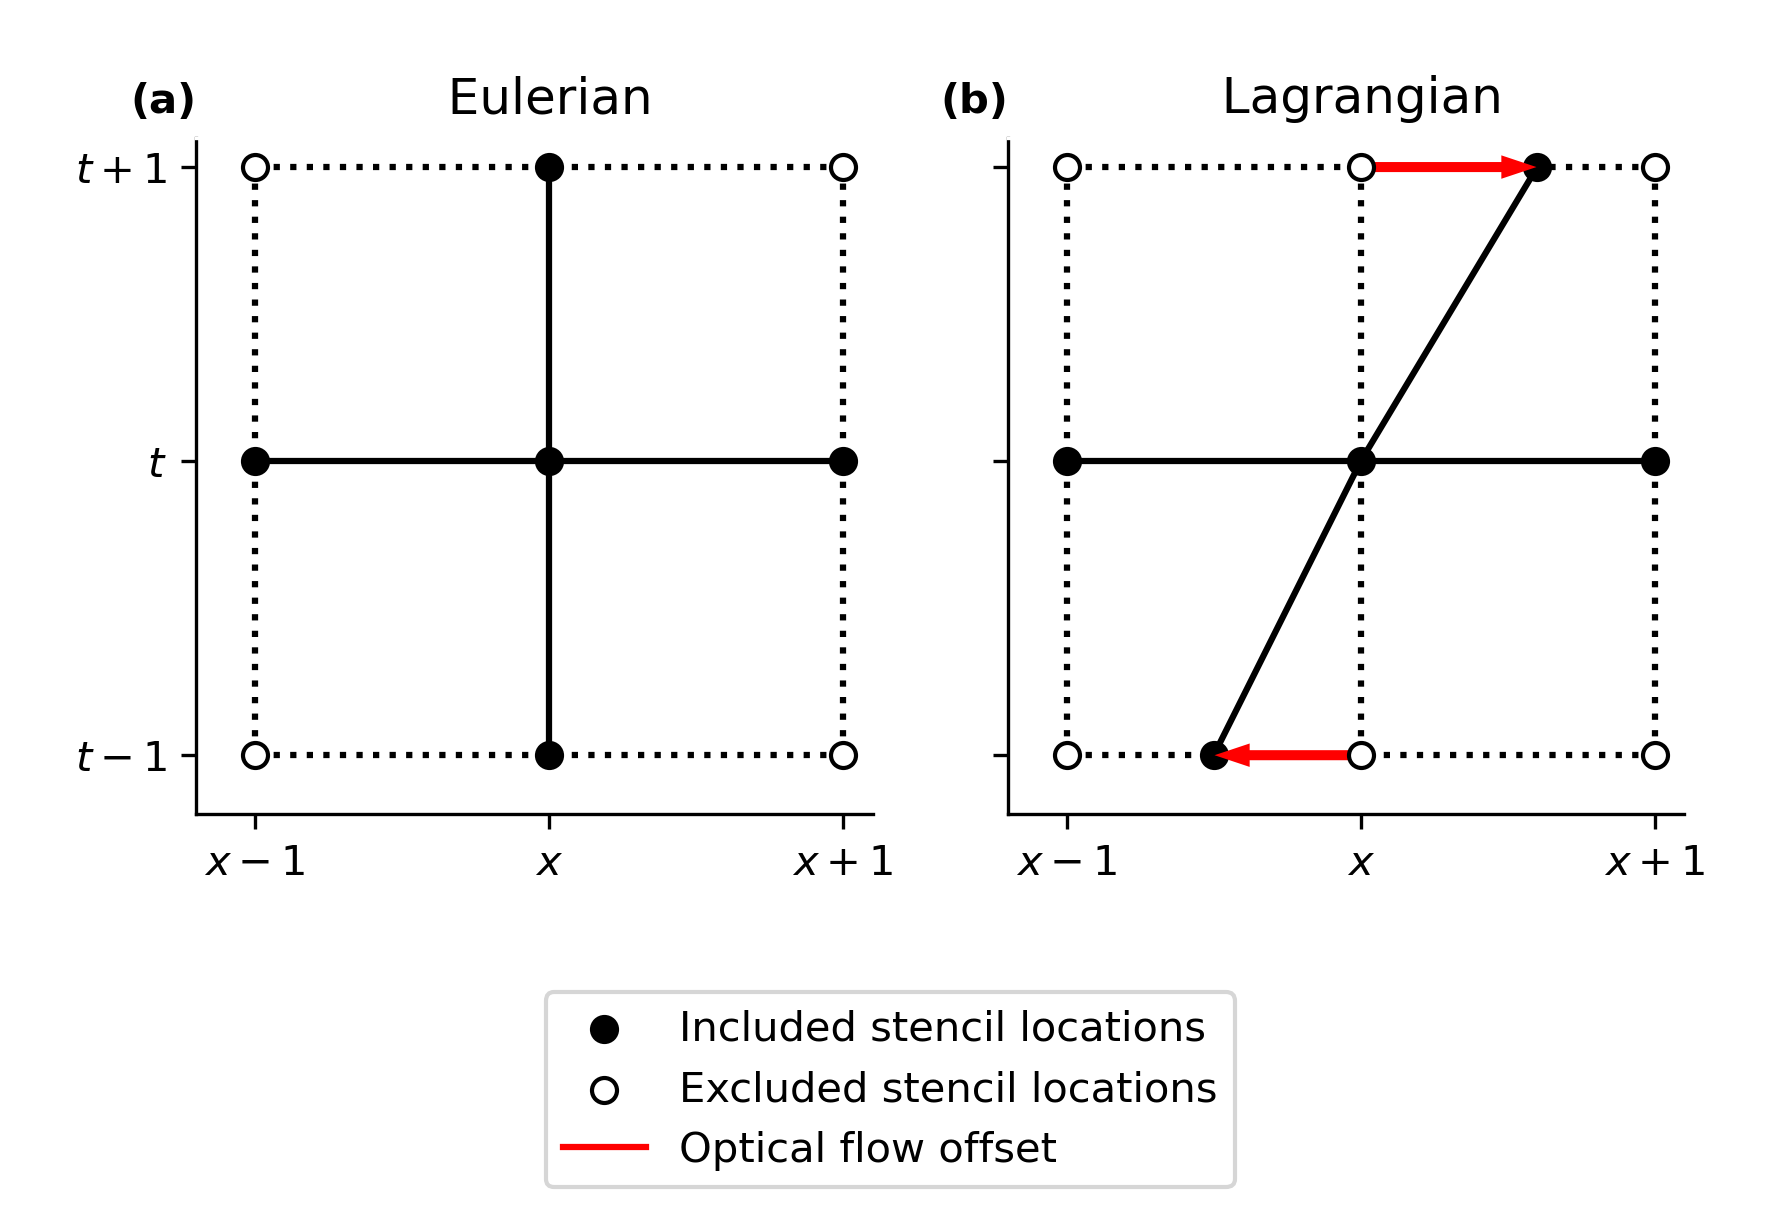
\includegraphics[width=0.75\textwidth]{figures/chapter1_15.png}
    \caption[
    A comparison of convolution stencils with square connectivity in Eulerian and Lagrangian frameworks.
    ]{
    A comparison of convolution stencils with square connectivity in Eulerian (a) and Lagrangian (b) frameworks. In the Lagrangian framework, the points at prior and subsequent time steps are offset by the calculated optical flow field.
    }
    \label{fig:convolution_kernels}
\end{figure}


To perform morphological operations which take into account this advection, a novel Lagrangian convolution method has been developed.
For spatial operations, the Lagrangian stencil operates identically to that of a classical convolution method.
However, when sampling points at prior or subsequent time steps, the locations of the stencil points are offset by the relevant optical flow vectors (fig.~\ref{fig:convolution_kernels}\,b).
Values at the offset stencil locations are interpolated, providing a Lagrangian reference frame for changes in the observations over time.
Applying the convolution stencil to every pixel in a sequence of images provides a semi-Lagrangian framework for morphological operations, combining the Lagrangian reference frame for evaluating changes over time while maintaining the regular grid of the images.

New implementations of several existing image processing operations have also been developed within the Lagrangian convolution framework, including:
\begin{itemize}
    \item Sobel edge detection \citep{sobel_isotropic_2014}
    \item Watershed segmentation using the connected-components method \citep{bieniek_efficient_2000}
    \item Labelling of connected components \citep{hoshen_percolation_1976}
\end{itemize}

These operations are used in this method to detect the full extent of the anvil cloud associated with the \acrshort{dcc}, to perform detection continuously across multiple time periods while accounting for the motion of the \acrshort{dcc}, and to identify individual \acrshort{dcc}s and \acrshort{dcc} clusters across multiple time periods respectively.

The Sobel method detects edges in an image using the magnitude of the local gradient at each pixel.
Edge detection enables the segmentation of an image into separate regions without pre-defined thresholds (such as in \acrshort{bt}) to separate them.

Watershed algorithms are a method of image segmentation that equates an image to a topographical map, with elevation according to the value of the pixel.
Each pixel is then descended towards its local minima until it reaches a predefined marker region.
The method takes its name from the geographical feature of the same name, which refers to the separation between adjacent drainage basins.
Although this physical interpretation of the algorithm applies to two-dimensional images, the method can be applied to arrays with any number of dimensions, such as the method used by \citet{fiolleau_algorithm_2013} which applied watershedding to a three-dimensional field.

Labelling algorithms assign unique identifiers to each segmented region provided by either the edge detection or watershed algorithms.


\subsection{Detection of Growing Deep Convection} \label{sec:core_detection}

Growing deep convective cores are detected in a similar manner to that used by \citet{zinner_cb-tram_2008}.
The growth rates are calculated using the finite difference of the 10.4\,\unit{\mu m } \acrshort{bt} and \acrshort{wvd} fields in the Lagrangian perspective.
Combining both the 10.4\,\unit{\mu m} \acrshort{bt} and the \acrshort{wvd} field provides the best observations for detecting growing deep convective cores.
The \acrshort{bt} field shows cooling cloud tops throughout the troposphere, while the \acrshort{wvd} isolates growth in the mid- to upper-troposphere, removing spurious observations of growth due to boundary layer convection and cloud formation.

A region of growing deep convection is classified as an area showing continuous cooling of greater than 0.5\,\unit{K} per minute in the 10.4\,\unit{\mu m} \acrshort{bt} field.
This growth rate must be detected over a minimum 15-minute period, covering an area of at least 3 by 3 pixels (approximately 7.5 by 7.5\,\unit{km}) at each time step.
Each region of detected growth is given a unique label, the average \acrshort{bt} of the detected cloud at each time step is calculated, and any label which fails to meet the cooling rate thresholds of 8\,\unit{K} over a 15-minute period (from \citep{roberts_nowcasting_2003, hartung_intercomparison_2013}) are removed.
Finally, each label is checked to ensure that the growth region ends with a \acrshort{wvd} field with a value of greater than -5, indicating that the growing core reaches a high altitude \citep{muller_role_2018}.
While threshold detection methods are sensitive to noise, the uncertainty in the \acrshort{bt} cooling rates due to sensor noise, combined with the uncertainty in the optical flow vectors, is not expected to exceed 5\% of the threshold.
A simple threshold method applied to the \acrshort{bt} cooling rate is, therefore, suitable for the detection of developing deep convection.

Figure~\ref{fig:core_detection} shows a comparison between the detected core cooling rates in \acrshort{abi} imagery and the corresponding column radar reflectivity measured by \acrshort{nexrad} for the case of newly developing convection (fig.~\ref{fig:core_detection}\,a,c,e) and mature \acrshort{dcc} (fig.~\ref{fig:core_detection}\,b,d,f)
Both 10.4\,\unit{\mu m} \acrshort{bt} and \acrshort{wvd} growth rates show growth detected in the same locations as the high column radar reflectivity from \acrshort{nexrad}.
As predicted by the results in section~\ref{sec:theory_core}, the observed growth rates in the \acrshort{wvd} are about half of those in the 10.4\,\unit{\mu m} \acrshort{bt}.


%f
\begin{figure}[tp]
    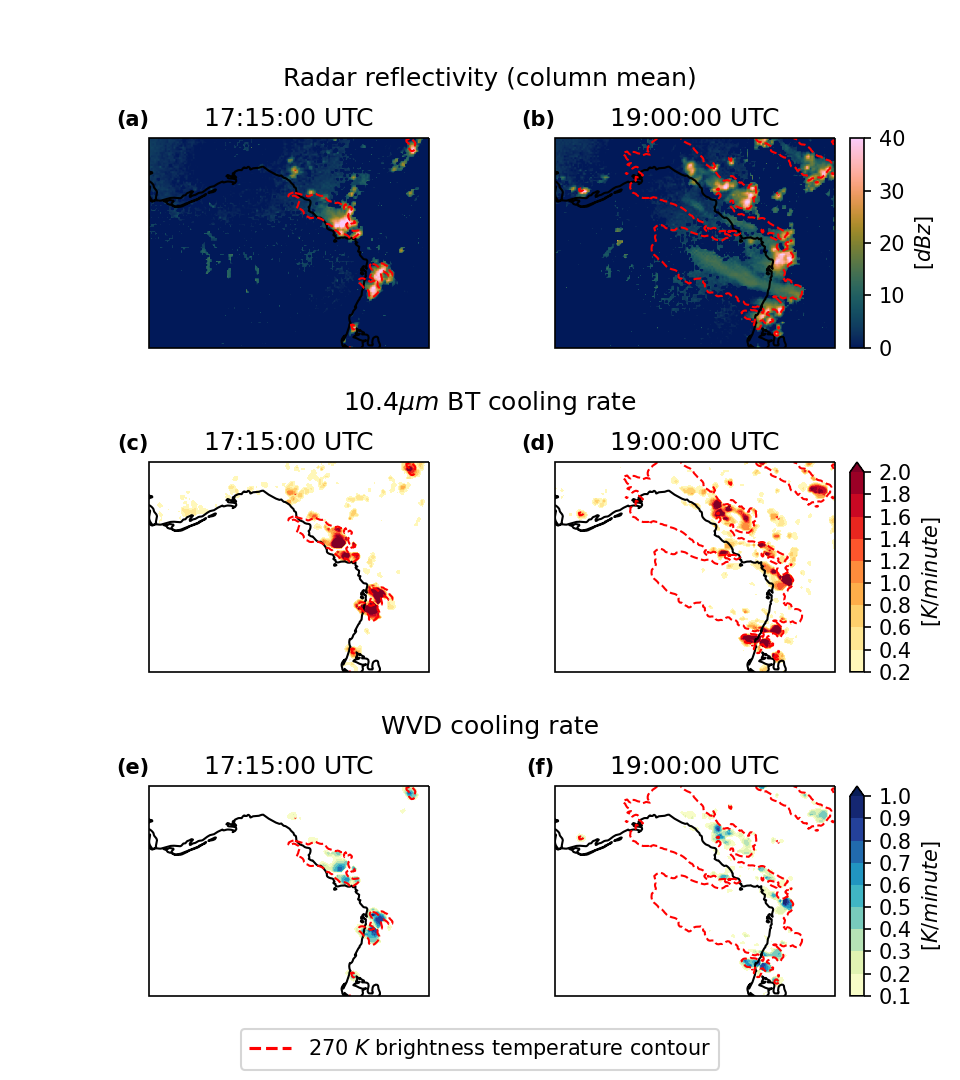
\includegraphics[width=\textwidth]{figures/chapter1_16.png}
    \caption[
    Detection of growing \acrshort{dcc} using \acrshort{nexrad} column radar reflectivity, 10.4\,\unit{\mu m} \acrshort{bt} and \acrshort{wvd} growth rates
    ]{
    Detection of growing \acrshort{dcc} regions for the \acrshort{dcc} cluster in figure~\ref{fig:compare_sat_radar_glm}. a,b: \acrshort{nexrad} column mean radar reflectivity remapped to the \acrshort{abi} grid. c,d: cooling rate of the 10.4\,\unit{\mu m} \acrshort{bt} field. e,f: warming rate of the \acrshort{wvd} field.
    }
    \label{fig:core_detection}
\end{figure}


Both 10.4\,\unit{\mu m} and \acrshort{wvd} growth rates in the growing phase (fig.~\ref{fig:core_detection}\,c,e) show good agreement with column radar reflectivity (fig.~\ref{fig:core_detection}\,a).
However, during the mature stage of the \acrshort{dcc}, discrepancies develop between the observed growth rates (fig.\ref{fig:core_detection}\,d,f) and the radar reflectivity (fig.~\ref{fig:core_detection}\,b) due to the development of the anvil cloud blocking satellite observations of the core underneath.


\subsection{Detection of Anvil Clouds} \label{sec:anvil_detection}

The region of anvil cloud associated with the growing convective clouds detected in section \ref{sec:core_detection} is detected and tracked using an edge-based watershed segmentation approach.
The edge-based approach to cloud detection avoids the use of a fixed threshold for anvil temperature, and so can detect a more accurate extent of the anvil cloud \citep{dim_alternative_2013}.
An upper threshold for the \acrshort{wvd} field of -5\,\unit{K} is defined, as used by \citet{muller_role_2018}, and a lower threshold of -12.5\,\unit{K}, which represents definite non-anvil cloud.
Because the presence of thin cirrus outflow from the anvil clouds can make it difficult to determine the extent of the anvil cloud, the \acrshort{swd} field is used as described in section 2.1 to either remove or include the region of cirrus outflow in the detected anvil region.
To detect the thick anvil cloud, the \acrshort{swd} field is subtracted from the \acrshort{wvd} field (fig.~\ref{fig:edge_detection}\,a).
In this case, the upper and lower thresholds remain the same as the \acrshort{swd} field is approximately 0~K for thick, high clouds, and so has no effect on the temperature of these features.
For detecting the thin anvil region, the \acrshort{swd} field is added to the \acrfull{wvd}, and the value of both thresholds is increased by 5\,\unit{K} to 0\,\unit{K} and -7.5\,\unit{K} respectively (fig.~\ref{fig:edge_detection}\,c).
This change is made to account for the effect of low-level \acrshort{wv} on the \acrshort{swd} field which gives a background value of approximately 5~K.
Between these two thresholds there is a region in which the extent of the anvil cloud is uncertain.
By applying a Sobel filter to detect the local gradient magnitude of the combined \acrshort{wvd}/\acrshort{swd} field \citep{sobel_isotropic_2014}, the outer extent of the anvil cloud is detected within this region where the greatest magnitude in the detected edges is found (see fig.~\ref{fig:edge_detection}\,b,d).

The uncertainty due to sensor noise is small relative to the range between the two thresholds, at 2.7\,\% for the combined \acrshort{wvd} and \acrshort{swd} fields.
While this low noise may indicate that a simple threshold approach may be suitable, such an approach would be susceptible to the systematic biases in the \acrshort{wvd} and \acrshort{swd} observations identified in section~\ref{sec:abi_channels}.
Combining the edge detection approach with the two-threshold approach provides robustness to systematic bias, since as long as the maximum gradient of the cloud edge remains between the two thresholds the same cloud extent should be detected.
This allows systematic biases on the order of several K without significantly affecting the results, allowing better comparison of \acrshort{dcc}s observed in different environments.


%f
\begin{figure}[tp]
    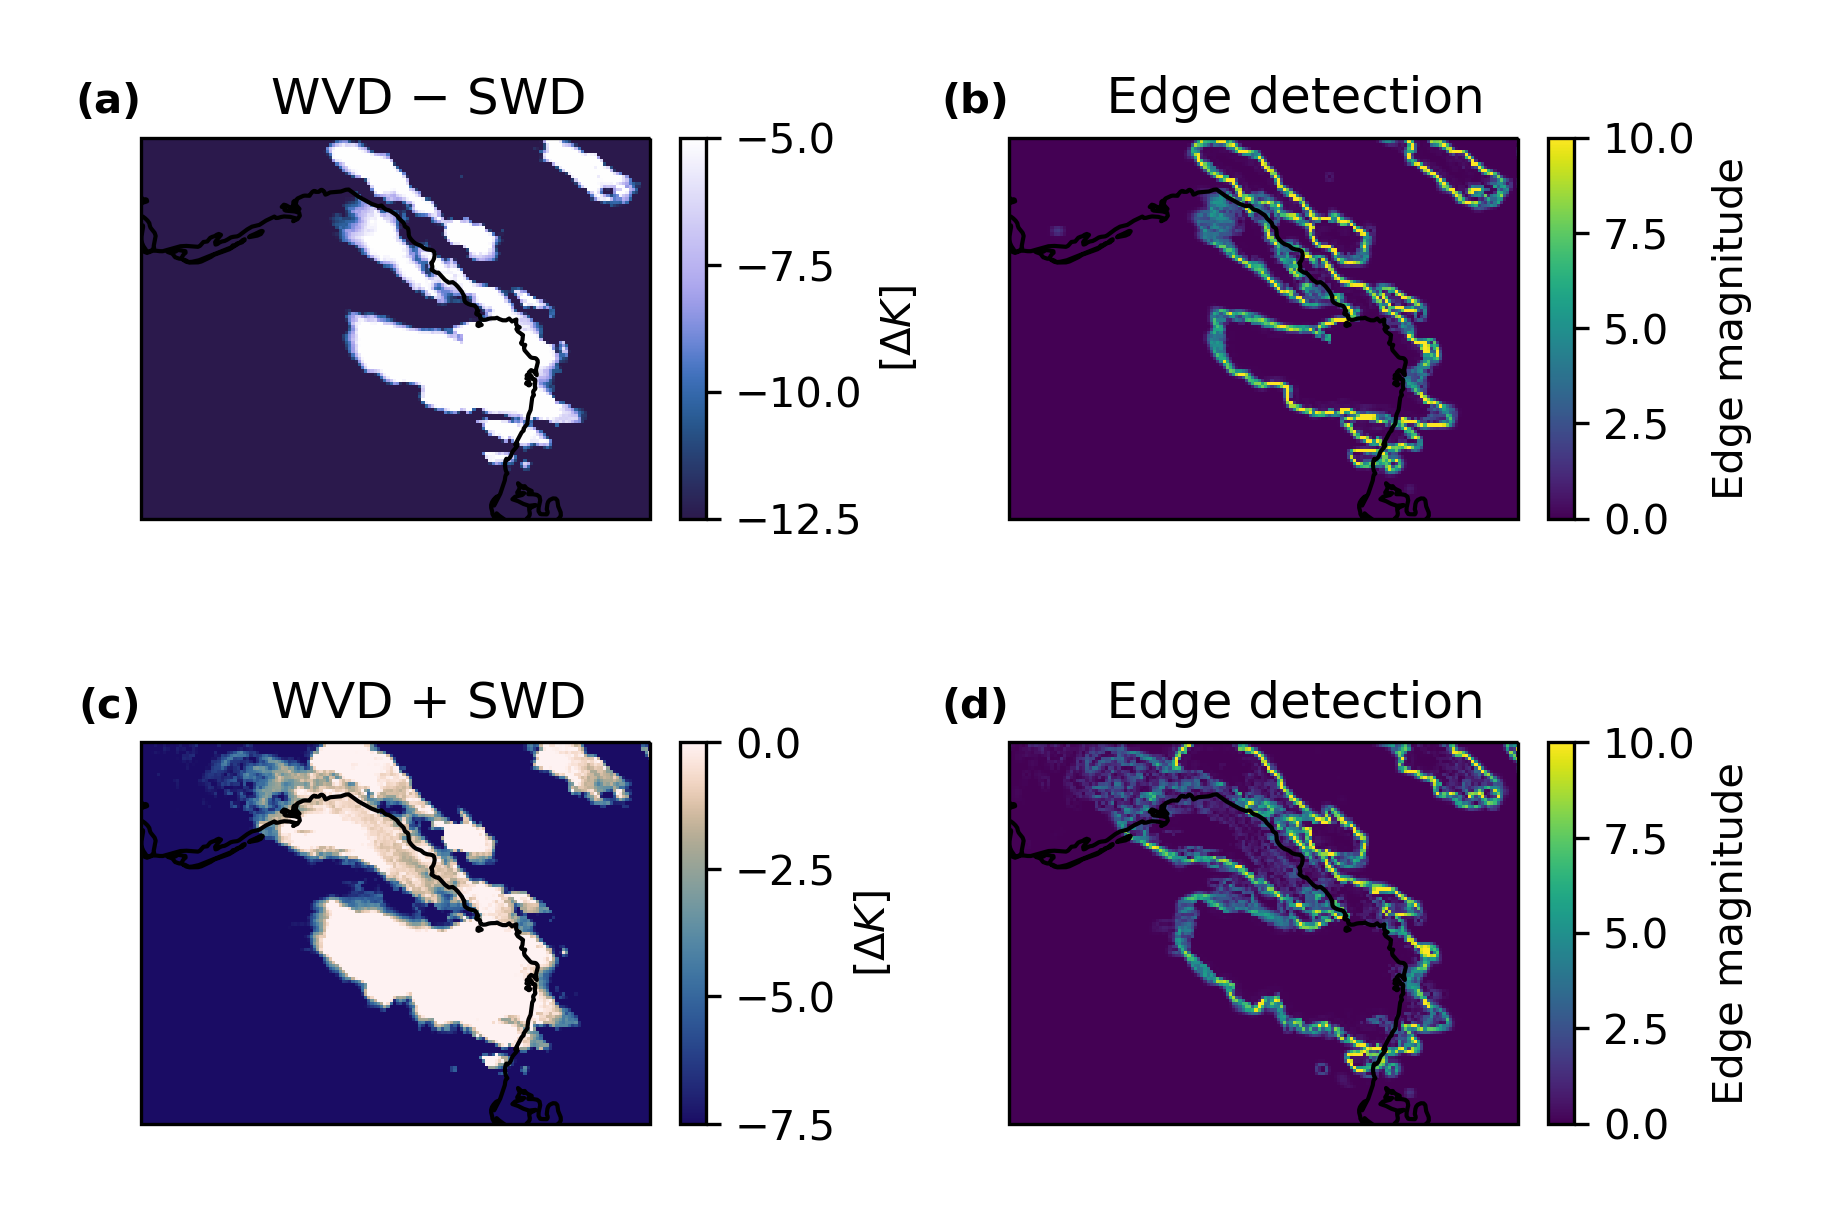
\includegraphics[width=\textwidth]{figures/chapter1_17.png}
    \caption[
    Detection of anvil cloud extent for the mature \acrshort{dcc} cluster in \ref{fig:compare_sat_radar_glm} using the edge gradient method
    ]{
    Detection of anvil cloud extent for the mature \acrshort{dcc} cluster in \ref{fig:compare_sat_radar_glm} using the edge gradient method. a.: The combined field of the \acrshort{wvd} minus the \acrshort{swd}, to isolate the thick anvil, between the upper and lower thresholds of -5 and -12.5\,\unit{K} respectively. b.: the detected edge gradient magnitude of the field between these thresholds, which is used to detect the outer extent of the thick anvil cloud. c.: the combined field of \acrshort{wvd} plus the \acrshort{swd}, to enhance the thin anvil, and d.: the calculated edge magnitude of this field.
    }
    \label{fig:edge_detection}
\end{figure}


When applied to the detected edges of the anvil clouds using the Sobel filter, with the growth regions detected previously as markers, the watershed method allows us to detect those anvil regions associated with detected regions of growing \acrshort{dcc}s, while avoiding the detection of non-convective regions of high, cold clouds.
Furthermore, due to the application of the watershed algorithm to both the spatial and temporal dimensions of the sequence of images through the semi-Lagrangian framework, the associated anvil clouds can be detected and tracked after the growth of the \acrshort{dcc} is no longer observed.

Figure~\ref{fig:detected_anvils} shows an example of the results of detecting and tracking \acrshort{dcc} cores (outlined in red) and the associated anvils (outlined in orange and blue for the thick and thin anvil regions respectively).
During the growing phase (fig.~\ref{fig:detected_anvils}\,a,b) a number of developing cores are seen, as well as the initial growth of primarily thick anvil cloud.
Figure~\ref{fig:detected_anvils}\,c--e shows the mature phase of the \acrshort{dcc}, where the thick anvil expands and the thin anvil cirrus starts to detrain towards the upper-left side of the figure.
Due to the anvil cloud reaching its maximum height, the initial developing cores seen in fig.~\ref{fig:detected_anvils}\,a,b are no longer detected as the cloud-top cooling cannot be observed.
Instead, new cores are detected developing on the edges of the anvil cloud.
In fig.~\ref{fig:detected_anvils}\,f--h, the detected anvil cloud begins to dissipate.
The thick anvil area decreases while the thin anvil area continues to increase as the anvil dissipates and detrains.
At this point in the lifetime of the tracked \acrshort{dcc} new growing cores are no longer observed, however the "3D" approach allows the continued tracking of the anvil cloud until it dissipates.


%f
\begin{figure}[tp]
    \centering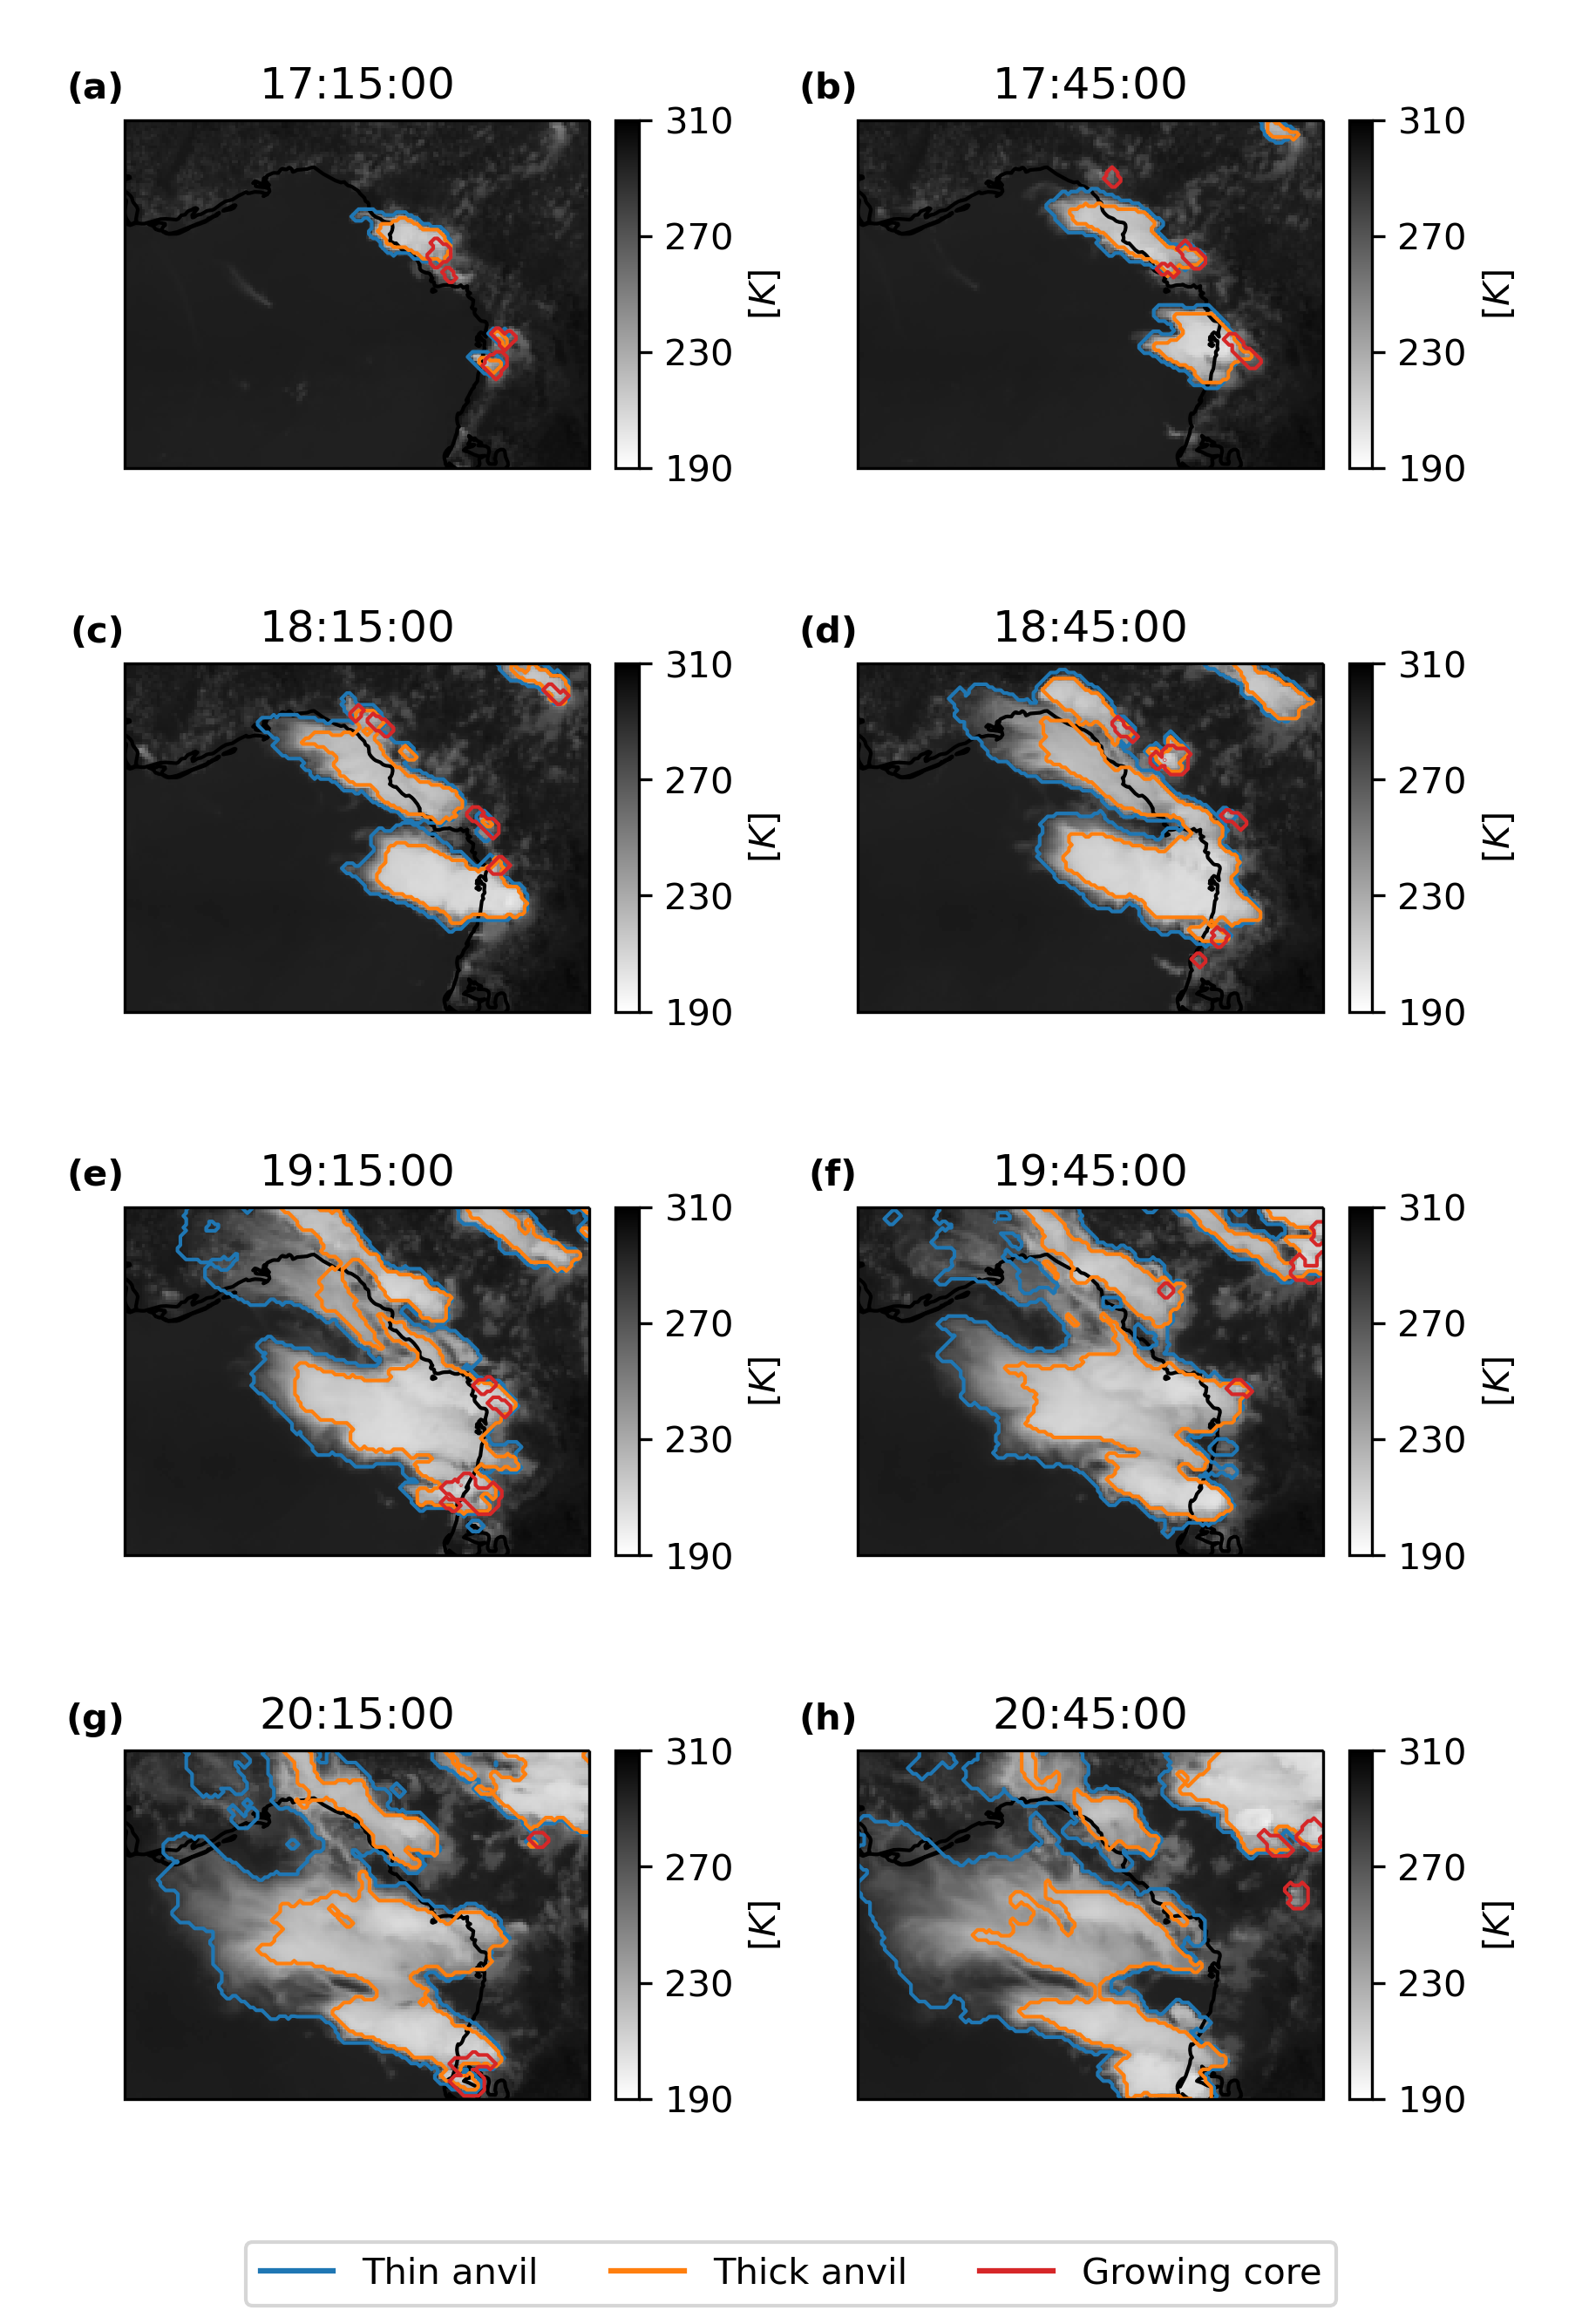
\includegraphics[width=0.8\textwidth]{figures/chapter1_18.png}
    \caption[
    Detected regions of thin anvil cloud, thick anvil cloud, and developing cores through the growing, mature and dissipating phases of the \acrshort{dcc} lifecycle
    ]{
    Detected regions of thin anvil cloud (blue), thick anvil cloud (orange), and developing cores (red) overlaid on the \acrshort{goes}-16 \acrshort{abi} 10.4\,\unit{\mu m} \acrshort{bt} field for the \acrshort{dcc} cluster from figure~\ref{fig:compare_sat_radar_glm}. The three stages of the \acrshort{dcc} lifecycle are shown; the growth phase (a,b), the mature phase (c--e), and the dissipating phase (f--g).
    }
    \label{fig:detected_anvils}
\end{figure}


\section{Evaluation}


The effectiveness of the semi-Lagrangian framework for the detection of \acrshort{dcc}s is evaluated by analysing the proximity of detected anvil cloud regions to lightning flash detection from \acrshort{glm}.
Lightning observations are frequently used to validate detection methods for deep convection \citep[e.g.][]{zinner_validation_2013, muller_novel_2019} due to the strong correlation between deep convective updraughts and lightning activity.
Although \acrshort{glm} is not capable of detecting all lightning events (approximately 70\% of lightning events are detected) \citep{peterson_removing_2020}, the high frequency of lightning flashes per \acrshort{dcc} mean that these observations provide a suitable ground truth for validation.
It should be noted that lightning observations are only suitable for validating the detection of the thick anvil region, as lightning does not occur in the cirrus outflow.
As a result, validation of the detection of the thin anvil region would require the use of other data such as cloud profiling radar or lidar observations, and is not considered further in this paper.


Here, the same validation method as that used by \citet{muller_novel_2019} to evaluate the semi-Lagrangian framework for the detection of \acrshort{dcc}s.
Detection events are classified into three categories:

\begin{itemize}
    \item Correct detection (CD), when the algorithm detects a \acrshort{dcc} that is collocated with one or more lightning observations
    \item False detection (FD), when the algorithm detects a \acrshort{dcc} but no lightning flash is observed
    \item Missed detection (ND), when the algorithm does not detect a \acrshort{dcc} but a lightning flash is observed
\end{itemize}

Using these three categories of events two measures of accuracy can be defined for the detection of \acrshort{dcc}s.
The \acrfull{pod} is defined as the number of correct detections divided by the total number of correct and missed detections.
This provides a measure of how likely the algorithm is to detect a \acrshort{dcc} that exists in the ground truth.
The \acrfull{far} is defined as the number of false detections divided by the total number of correct and false detections.
This provides a measure of how likely a \acrshort{dcc} detected by the algorithm is not present in the ground truth.
The F\textsubscript{1}-score is calculated as the harmonic mean of the \acrshort{pod} and the recall (where the recall in is 1~\textminus~\acrshort{far}), and provides an overall measure of accuracy between 0 and 1.

When evaluating whether detected \acrshort{dcc} regions and lightning observations were collocated, \citet{muller_novel_2019} considered events within 32\,\unit{km} and 15 minutes to be collocated.
This margin of uncertainty was separated into two components, half from the physical separation between observed lightning strikes, and the remaining half from uncertainty in the collocation and geolocation of the satellite and lightning observations.
For a typical \acrshort{abi} pixel length over the \acrshort{conus} of 2-2.5\,\unit{km}, this margin of error translates into 15 pixels in the \acrshort{abi} view.
The distance between a \acrshort{glm} lightning flash and detected cloud region is defined as the distance between the flash and the nearest \acrshort{abi} pixel within that region, with \acrshort{glm} flashes that fall within a detected \acrshort{dcc} given a distance of 0.
When considering that the resolution of \acrshort{glm} is a factor of four less than that of \acrshort{abi}, the same justification for the margin of error used by \citet{muller_novel_2019} is also applicable to collocated observations from \acrshort{abi} and \acrshort{glm}.

Validation was performed using \acrshort{goes}-16 \acrshort{abi} data from the \acrshort{conus} scan region for the entirety of 2018, which was processed using the method described in this chapter.
In total validation was performed for 319 days of \acrshort{abi} data, the remaining 46 days being excluded due to missing observations from either the \acrshort{abi} (1 day) or \acrshort{glm} (45 days) instruments aboard \acrshort{goes}-16.
Detection and tracking of \acrshort{dcc}s was performed over the \acrshort{conus} scan region of \acrshort{abi} for daily periods. 
By performing validation over both a large region, including a range of both land and ocean domains, and a full year time period, any bias in the validation associated with the variability of the accuracy of the method with location and season is avoided.

%t
\begin{table}[tb]
\centering
\begin{tabular}{lcrrr}
\tophline
Detection Method            & n         & \acrshort{pod}    & \acrshort{far}    & F\textsubscript{1}-score \\ 
\middlehline
Growth-based                & 598,038   & 0.4017            & 0.2136            & 0.5318  \\
\acrshort{wvd} threshold    & 678,854   & 0.9727            & 0.6457            & 0.5194  \\
Semi-Lagrangian             & 145,969   & 0.9837            & 0.1611            & 0.9056 \\
\bottomhline
\end{tabular}
\caption[
\acrshort{pod}, \acrshort{far} and F\textsubscript{1}-score for three different detection methods validated against observed \acrshort{glm} flashes
]{
\acrshort{pod}, \acrshort{far} and F\textsubscript{1}-score for three different detection methods validated against observed \acrshort{glm} flashes (n=116,671,289). Growth-based refers to the detection of growing \acrshort{dcc}s using the method described in section \ref{sec:core_detection} \acrshort{wvd} threshold uses the threshold method developed by \citet{muller_role_2018}. Semi-Lagrangian refers to the detection of anvil clouds connected to growing cores using the edge-based watershedding method described in section \ref{sec:anvil_detection}.
} % Table Footnotes
\label{table:validation}
\end{table}


Results of the validation of the detected anvil region, as well as those for the detection of growing deep convection and the \acrshort{wvd} filter, are shown in table \ref{table:validation}.
The regions of growing \acrshort{dcc}s detected using the method described in section \ref{sec:core_detection} shows low scores for both the \acrshort{far} and \acrshort{pod} metrics.
While the detection of growing \acrshort{dcc}s shows a low \acrshort{far} of 0.21, the short time frame in which growth can be observed leads to a high rate of missed detections of lightning flashes, which results in a \acrshort{pod} of 0.40.
This is not necessarily because the algorithm fails to detect cores, but because many lighting observations occur during the mature phase of convection (see fig.~\ref{fig:compare_sat_radar_glm}\,h, \ref{fig:dcc_over_time}\,d), and these lightning flashes are not detected as the core is only observed during the growing phase.

For comparison, the accuracy of detecting anvils only by a fixed threshold of the \acrshort{wvd} without detecting growing cores is also evaluated, as used by \citet{muller_role_2018}.
Compared to the detection of growing \acrshort{dcc} regions, the \acrshort{wvd} threshold shows a much higher \acrshort{pod} of 0.97, but also has a high \acrshort{far} of 0.64, repeating the findings of \citet{muller_novel_2019} which show that although the \acrshort{wvd} threshold method is capable of detecting the majority of \acrshort{dcc}s, it is incapable of distinguishing between anvil clouds and other thick, high altitude clouds.
Furthermore, the \acrshort{wvd} threshold detection detects a larger number of objects (n=678,854) compared to either of the other detection methods, further indicating that a large number of non-convective clouds are detected using the threshold method on its own.
Note that both the core detection and \acrshort{wvd} threshold approach have similar F\textsubscript{1}-scores (0.53 and 0.51 respectively) as both prioritise one measure of accuracy over the other.

Finally, the anvil regions detected using a combination of the detected growth regions and the \acrshort{wvd} field using the semi-Lagrangian framework described in section \ref{sec:anvil_detection} are validated.
The novel method has a high \acrshort{pod} of 0.98 similar to that of the \acrshort{wvd} threshold, while also maintaining much of the low \acrshort{far} of the detection of growing \acrshort{dcc}s (\acrshort{far}=0.16).
As a result, the semi-Lagrangian method displays a high overall F\textsubscript{1}-score of 0.91.
This result highlights the capability of the semi-Lagrangian detection framework to use growth-based detection methods to substantially reduce the compromise between \acrshort{pod} and \acrshort{far} error rates by combining multiple methods for the detection of \acrshort{dcc}s.


\section{Summary}  %% \conclusions[modified heading if necessary]

Algorithms for the detection and tracking of \acrshort{dcc}s perform a vital role in both forecasting and research applications.
Sequences from geostationary satellites provide unique observations of \acrshort{dcc} anvil clouds over their entire lifecycle.
However, the traditional framework used by such algorithms requires a compromise between the rates of false and missed detections due to the overlap in signature from convective and non-convective clouds \citep{konduru_new_2013}.
Whereas novel methods have approached this problem for the detection of large, mesoscale convective systems \citep{fiolleau_algorithm_2013}, such approaches do not take advantage of the capability of the latest generation of geostationary imaging satellites to detect individual deep convective cores.

By developing and implementing a novel semi-Lagrangian framework for the detection and tracking of \acrshort{dcc}s, the detection of growing \acrshort{dcc} cores \citep{zinner_cb-tram_2008} and \acrshort{dcc} anvils \citep{muller_role_2018} to detect and track \acrshort{dcc}s over their entire lifecycles can be combined.
The novel methods developed here for the semi-Lagrangian computer vision framework, along with implementations of multiple image processing operations commonly used for object detection, allow the accurate detection and tracking of moving objects utilising both spatial and temporal information.
These methods may have impacts on applications of computer vision beyond the detection and tracking of \acrshort{dcc}s.
Furthermore, the novel framework can achieve higher levels of accuracy without compromising on the number of \acrshort{dcc}s detected, as with previous algorithms \citep{muller_novel_2019}.

Using this novel methodology, both small, isolated \acrshort{dcc}s and large, mesoscale convective systems can be detected and tracked with a high degree of accuracy, high spatial and temporal resolution and across large domains such as the \acrshort{conus}.
The data provided about the behaviour of \acrshort{dcc}s over their entire lifetime will allow new research into vital topics such as the response of deep convection and climate change, and the interactions and feedbacks between \acrshort{dcc}s and large-scale atmospheric thermodynamics \citep{varble_erroneous_2018}.

